\chapter{Foundations}
\label{chapter:preli}
\textit{``The beginning of knowledge is the discovery of something we do not understand''}- Frank Herbert 

\section{Chapter Overview}
In this chapter, we cover the foundations and concepts that will be found in all the subsequent chapters. We start with a basic DSS and move towards an intelligent DSS. Subsequently, we cover the necessary foundations for building an explainable decision support system~(DSS) to provide diagnosis for cancer. In particular, we cover in detail the concepts of machine learning~(ML) and deep learning~(DL), explainable artificial intelligence~(XAI), decision rules, neuro-symbolic reasoning, and representation learning, with a focus on explainability and algorithmic transparency. However, more detailed definitions, chapter wise contributions, results, and focused related work are included in subsequent chapters. Later in the chapter, we discuss different types and subtypes of cancer, growth and metastasis of cancer, in order to know the biological interpretations of genomics data. 

\section{Decision Support Systems}\label{sec:DSS}
A DSS is an information system that supports business or organizational decision-making activities. A typical DSS is takes a set of input, e.g., factors, numbers, and characteristics to analyze and transforms data from which DSS `decisions' are generated. Finally, results generated by the DSS based on user criteria, which is often annotated or validated with User knowledge and expertise. In other words, a DSS is  often a computerized program assists which sifts through and analyzes massive amounts of data, compiling comprehensive information that can be used to solve problems and in decision-making. DSS components can be broadly classified as follows~\cite{hackathorn1981organizational}: 

\begin{enumerate}[noitemsep]
    \item  \textbf{Inputs}: Factors, numbers, and characteristics to analyze.
    \item \textbf{Knowledge base}: Inputs requiring manual analysis by the user.
    \item \textbf{Outputs}: Transformed data from which DSS "decisions" are generated.
    \item \textbf{Decisions}: Results generated by the DSS based on user criteria.
\end{enumerate}

\hspace*{3.5mm} Three fundamental components of a DSS architecture includes a knowledge base~(KB), a model~(decision context and user criteria), and an a user interface. Besides, users themselves are important components of the architecture. Using the relationship with the user as the criterion,  Haettenschwiler et al.~\cite{haettenschwiler1999neues} differentiates passive, active, and cooperative DSS:  

\begin{itemize}[noitemsep]
    \item \textbf{A passive DSS}: it can aid the process of decision making, but cannot bring out explicit decision suggestions or solutions.
    \item \textbf{An active DSS}: it can bring out decision suggestions or solutions. 
    \item \textbf{A cooperative DSS}: it allows for an iterative process between human and system towards the achievement of a consolidated solution.
\end{itemize}

\hspace*{3.5mm} A cooperative system has several advantages over active and passive DSS. For example, using a cooperative DSS, decision makers can modify or refine the decision suggestions provided by the system, before sending them back to the system for validation. Subsequently, the system again improves, completes, and refines the suggestions of the decision maker and sends them back to them for validation. Besides, D. Power et al.~\cite{power2002decision} has differentiated communication-driven DSS, data-driven DSS, document-driven DSS, knowledge-driven DSS, and model-driven DSS, according to the mode of assistance~\cite{power2002decision}:

\begin{itemize}[noitemsep]
    \item \textbf{A communication-driven DSS}: it enables cooperation, supporting more than one person working on a shared task; examples include integrated tools like Google Docs. 
    \item \textbf{A data-driven DSS}: it emphasizes access to and manipulation of a time series of internal company data and, sometimes, external data.
    \item \textbf{A document-driven DSS}: it manages, retrieves, and manipulates unstructured information in a variety of electronic formats.
    \item \textbf{A knowledge-driven DSS}: provides specialized problem-solving expertise stored as facts, rules, procedures or in similar structures like interactive decision trees and flowcharts.
    \item \textbf{A model-driven DSS:} emphasizes access to and manipulation of a statistical, financial, optimization, or simulation model. Model-driven DSS use data and parameters provided by users to assist decision makers in analyzing a situation; they are not necessarily data-intensive. 
\end{itemize}

\hspace*{3.5mm} On the other hand, a DSS that can perform selected cognitive decision-making functions based on artificial intelligence~(AI) or intelligent agents technologies called intelligent DSS. Owing to outstanding performance across domains such as computer vision, natural language processing, multimedia analytics, and business analytics, AI-guided DSS could eventually be applied to various automated decision-making process. In an AI-guided or intelligent DSS, a set of learning algorithms are embedded to perform cognitive decision-making in which ML often act as one of the most common forms of AI. 
%However, DNN models are perceived mostly as `black box' methods because of their not well-understood internal functioning. Besides, they cannot reason their underlying decisions, leaving them incapable of aiding transparent and trustworthy decisions. Consequently, we call such DSS a `black box' model. 
Since we aim to improve the transparency and explainability of such intelligent but black-box DSS throughout this thesis, we now focus on the fundamental components such as ML, DL, representation learning, and multimodal learning. Then we will discuss about the need for interpretability. 
%This chapter provides a general introduction to this dissertation, provides the motivation for this research, list down the hypotheses and research questions, and outlines the structure of this thesis. 

\section{Machine Learning}
ML is about using a set of statistical and mathematical algorithms to perform tasks such as concept learning, predictive modeling, clustering, and mining useful patterns can be performed, where a learner or ML algorithm is the program used to learn a ML model from data. Subsequently, a ML model is the learned program that maps inputs to predictions. Tom M. Mitchell~\cite{mitchell1997machine} explained what learning really means from a computer science perspective: \textit{``a computer program is said to learn from experience $E$ with respect to some class of tasks $T$ and performance measure $P$, if its performance at tasks in $T$, as measured by $P$, improves with experience $E$"}. We can interpret the above definition in another way: based on a set of observation or data~(i.e., experience $E$), a learning algorithm can be used to solve a problem~(i.e., task $T$) iteratively, i.e., as long as the performance~(i.e., $P$) is not satisfactory. 

\hspace*{3.5mm}Based on this interpretation, a machine can learn from data/observations and can be improved with experience to predict an outcome more accurately. When it comes to data, what we mean is a set of features/inputs and targets from which the machine learns. Subsequently, a learned program called a ML model can map inputs to predictions. The resultant is weights for a linear model or for a neural network~(we'll shortly discuss about). Training a ML model is an optimization problem, where the primary objective is finding a minimizer of a convex function $f$ and a weight vector $w$ on $d$ data points. We can formulate it as $\min _{w \in \mathbb{R}^{d}} f(w)$, where the objective function is as follows~\cite{karim2018scala}:

\vspace{-4mm}
\begin{align}
    f(w):=\lambda R(w)+\frac{1}{n} \sum_{i=1}^{n} L\left(w ; x_{i}, y_{i}\right)
\end{align}

\hspace*{3.5mm} We call the method linear if $L(w;x,y)$ can be expressed as a function of $w^Tx$ and $y$. The objective function $f$ has two components, i) a regularizer that controls the complexity of the model, ii) the loss that measures the error of the model on the training data. The loss function $L(w;)$ is typically a convex function in $w$. The fixed regularization parameter $\lambda \geq 0$ defines the trade-off between minimizing the loss on the training error and minimizing model complexity to avoid overfitting~\cite{karim2018scala}. If both of components are convex, their sum is also convex, else non-convex~\cite{zaccone2018deep}. Therefore, using a convex optimization technique, we can minimize the function until it converges towards the minimum error.  %This can be a set of weights for a linear model or for a neural network. Other names for the rather unspecific word "model" are "predictor" or - depending on the task - "classifier" or "regression model". he trained ML model is called $\hat{f}$ or $\hat{f}(x)$

\begin{figure}[h]
	\centering
	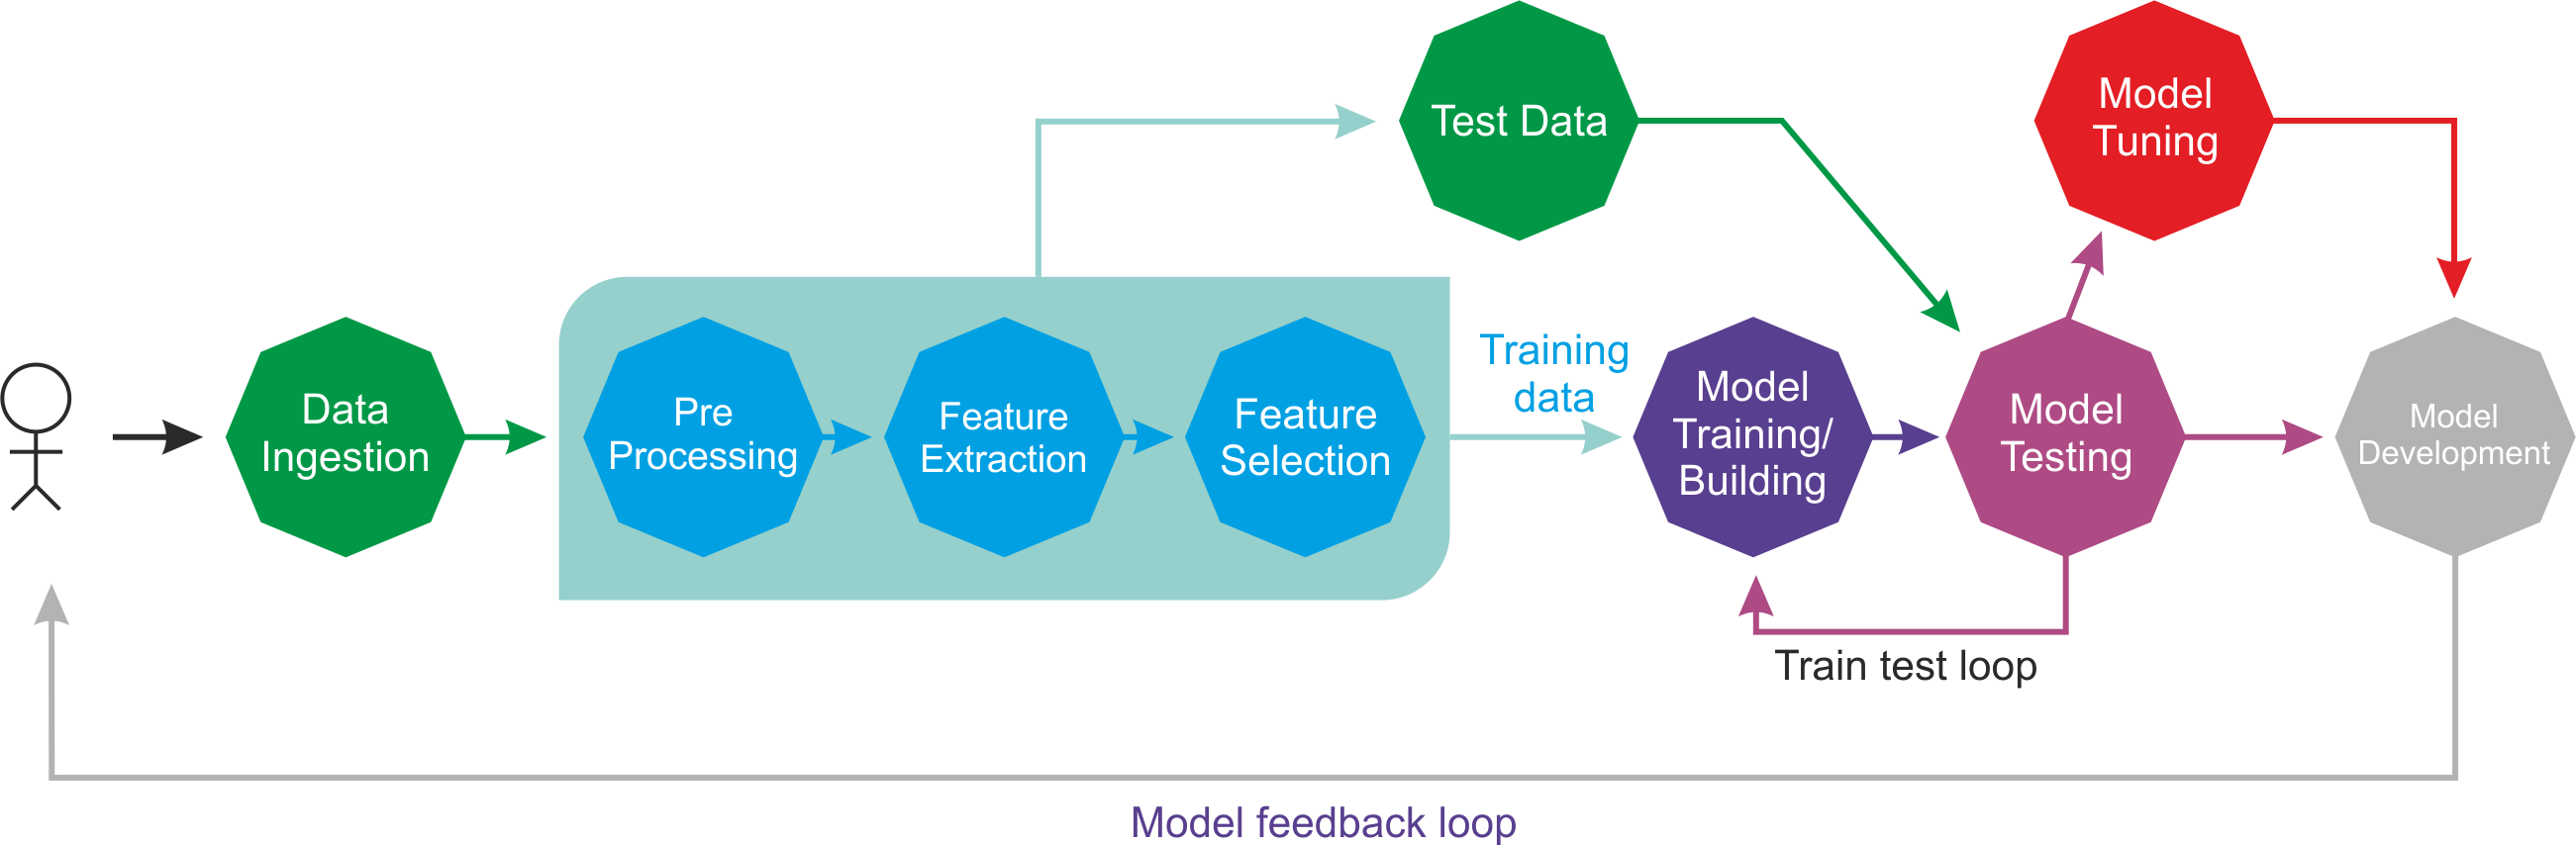
\includegraphics[width=0.9\linewidth,height=60mm]{images/B08452_01_02.png}
	\caption{Lifecycle of a typical ML pipeline~\cite{karimScalaML2019}} 
	\label{fig:ml_pipeline}
\end{figure}

\hspace*{3.5mm} The regularization parameter defines the trade-off between minimizing the training error and the model's complexity in an effort to avoid overfitting problems. More elaborately, when using an ML algorithm, the goal is to obtain the best hyperparameters of a function that return the minimum error when making predictions. 
%Given that a problem is convex, it is usually easier to analyze the asymptotic behavior of the algorithm, which shows how fast it converges as the model observes more and more training data. 
The challenge of ML is to allow training a model so that it can recognize complex patterns and make decisions not only in an automated way but also as intelligently as possible. 
However, if the performance is not satisfactory, additional tuning or retraining would be necessary to get the best model, before % based on hyperparameter optimization.
deploying the best model in a production-ready environment. 
\Cref{fig:ml_pipeline} summarizes these steps in a nutshell. 

\vspace{2mm}
\begin{tcolorbox}[colback=white!3!white,colframe=gray!120!black,title=\faBook~Data instance and prediction:]
    %INFO: \faBook \\
    \scriptsize{
        \textbf{An instance}: is a row in the dataset~(also called data point, example, or observation). An instance consists of the features $x^{(i)}$ and~(if known) the target outcome ${y}$, where target is the information that the model learned to predict. \\
        \textbf{Prediction:} is what a ML model ``guesses" what the target value should be based on the given feature, i.e., $\hat{y}$ = $\hat{f}\left(x^{(i)}\right)$. If $\hat{y}$ is equal to~(or close) ${y}$, we say it's an accurate prediction.   
        }
\end{tcolorbox}

\subsection{Machine learning tasks}
Although every ML problem is more or less an optimization problem, the way they are solved can vary. Depending on the data type~(often combination of features and targets), learning tasks could be of different three types such as supervised, unsupervised, and reinforcement learning. Supervised learning is the simplest and most well-known automatic learning task. It is based on a number of predefined examples, in which the category to which each of the inputs should belong is already known, as shown in \cref{fig:ml_pipeline_sup}:

\begin{figure}[h]
	\centering
	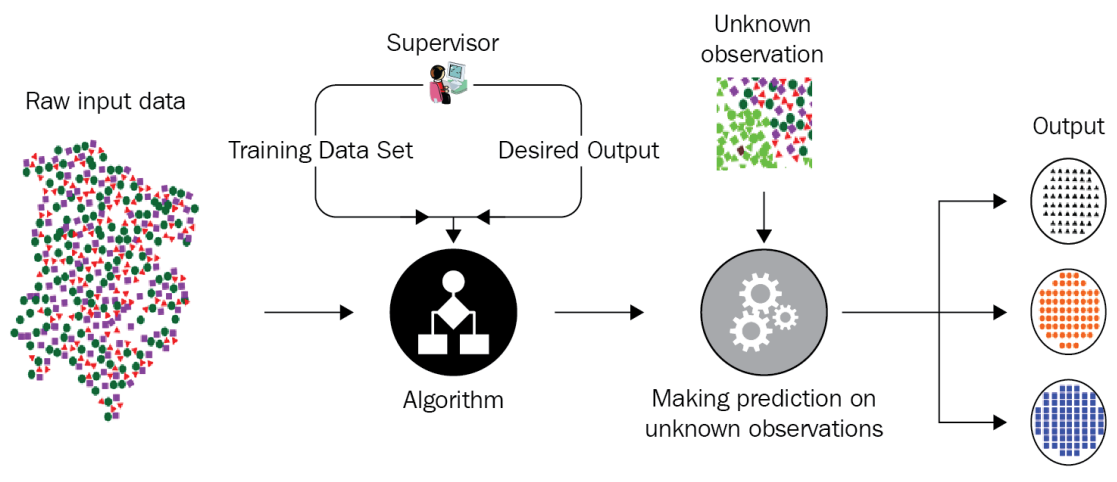
\includegraphics[width=0.9\linewidth,height=50mm]{images/sup.png}
	\caption{Workflow of supervised learning technique~\cite{karimScalaML2019}} 
	\label{fig:ml_pipeline_sup}
\end{figure}

\hspace*{3.5mm} In the preceding diagram, an actor~(e.g., data scientist) performs extraction, transformation, and load~(ETL) and necessary feature engineering~(such as feature extraction, selection, etc.) to get the appropriate data consisting of features and labels, to fed into the model. The training set is used to train a ML model and the validation set is used to validate the training against the overfitting problem and regularization. Then the actor can evaluate model's performance on the test set~(i.e., unseen data). The supervised learning context includes classification and regression. 

\vspace{2mm}
\begin{tcolorbox}[colback=white!3!white,colframe=gray!120!black,title=\faBook~Classification vs. regression:]
    %INFO: \faBook \\
    \scriptsize{
        \textbf{Classification:} it is used to predict which class a data point is a part of discrete value or the label of the class attribute. \\
        \textbf{Regression:} it is used for predicting continuous values and making a numeric prediction of the class attribute.
        } \\
\end{tcolorbox}

\hspace*{3.5mm} How would you summarize and group a dataset if the labels were not given? Probably, you'll try to answer this question by finding the underlying structure of a dataset and measuring the statistical properties such as frequency distribution, mean, standard deviation, and so on. If the question is how would you effectively represent data in a compressed format? You'll probably reply saying that you'll use some software for doing the compression, although you might have no idea how that software would do it. \Cref{fig:ml_pipeline_unsup} shows the typical workflow of an unsupervised learning task. 

\begin{figure}[h]
	\centering
	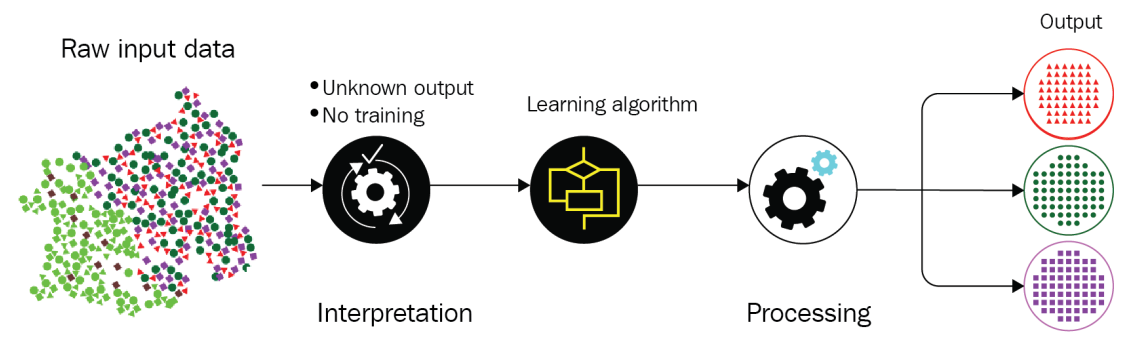
\includegraphics[width=0.9\linewidth,height=50mm]{images/unsup.png}
	\caption{Workflow of unsupervised learning technique~\cite{karimScalaML2019}} 
	\label{fig:ml_pipeline_unsup}
\end{figure}

\hspace*{3.5mm} On the other hand, reinforcement learning focuses on the learning of the system through its interactions with the environment, where system's parameters are adapted based on the feedback obtained from the environment, which in turn provides feedback on the decisions made by the system. On the other hand, another most complex forms of ML involve deep learning~(DL), or deep neural network~(DNN) models with many levels of features or variables that predict outcomes that help take meaningful decision. We will discuss about DL and DNN in subsequent sections. 

%The following diagram shows a person making decisions in order to arrive at their destination. 

%After necessary preprocessing and feature engineering, a common practice is splitting the input data into 60\% for the training, 10\% for the validation, and 20\% for testing, but it depends on use cases. \hspace*{3.5mm} Besides, up-sampling or down-sampling may require in case of class imbalanced scenario. In practice and from the application point of view, a typical ML application involves several processing steps, from the input to the output, forming a scientific workflow as shown \cref{fig:ml_pipeline}. 

\subsection{Role of data in machine learning}
Data in any ML pipeline is a first-class citizen and play key role. The performance of any learning depends on quality features. Depending upon the learning tasks, often we may have to split the data, e.g., in supervised learning tasks, the entire learning process requires input datasets to split into different sets~\cite{karim2018java}:

\vspace{-1mm}
\begin{itemize}[noitemsep]
    \item \textbf{Training set:} is the knowledge base coming from historical or live data used to fit the parameters of the ML algorithm. During the training, the model utilizes the training set to find optimal weights of the network and reach the objective function by minimizing the training error~\cite{karim2018java}. 
    \item \textbf{Validation set:} is a set of examples used to tune the parameters of an ML model to ensure that the model generalizes towards avoiding overfitting~\cite{karim2018java}. 
    \item \textbf{Test set:} is used for evaluating the performance of the trained model on unseen data. This step is also referred to as model inferencing. After assessing the final model on the test set, no need to tune the model before deploying in a production-ready environment~\cite{karim2018java}.
\end{itemize}
\vspace{-1mm}

\hspace*{3.5mm} In the context of supervised learning, the learning process required for the input dataset is split randomly into three sets, for example, $60\%$ for the training set, $10\%$ for the validation set, and the remaining $30\%$ for the testing set.

\section{Deep Learning and Neural Networks}
Deep neural networks~(DNNs) form the core of deep learning~(DL) by providing a set of algorithms to model complex and high-level abstractions in data and can better exploit large-scale datasets to build complex models, and have been widely used in computer vision, speech recognition, NLP, social network, machine translation, bioinformatics, etc. Layers in a neural network is composed of a set of artificial neurons called perceptron~\cite{yuan2019adversarial}. A perceptron maps a set of inputs to outputs with a special function called activation functions. Multiple such layers are stacked to create such a neural network. 

\hspace*{3.5mm} Till date, numerous neural network architectures have been proposed and are in use. We can categorize DL architectures into four groups: i) feed-forward neural networks~(FFNNs), ii) Convolutional neural networks~(CNNs), iii) Recurrent neural networks~(RNNs), iv) Autoencoders~(AEs), and v) Emergent architectures. However, FFNNs, CNNs, AEs, and RNNs have many improved variants. Although most of the variants are proposed or developed for solving domain-specific research problems, the basic working principles still follow the original  architectures. In this section, we provide preliminaries and theoretical foundations of these architectures that are used throughout in the subsequent chapters.  

\subsection{Feed-forward neural networks}
Feed-forward neural networks~(FFNNs) are neural networks that have a complex and deeper architecture with a large number of neurons in each layer, and many connections between them. Although DNN refers to a very deep network, for simplicity, we consider MLP, stacked autoencoder~(SAE), and deep belief networks~(DBNs)~\cite{Hinton:2009} as DNN architectures. These architectures mostly work as an FFNN, meaning information propagates from input to output layers. Multiple perceptrons are stacked together as MLPs, where layers are connected as a directed graph. Fundamentally, an MLP is one of the most simple FFNNs since it has three layers as shown in \cref{fig:mlp_1}: an input layer, a hidden layer, and an output layer, where the signal propagates one way, from the input layer to the output layer as shown in \cref{fig:mlp_1}.

\hspace*{3.5mm} However, it is not possible to determine a priori, with adequate precision, the required number of hidden layers, or even the number of neurons that must be contained inside each hidden layer to compute a non-linear function. There is no straightforward answer to this, but we can try increasing the number of neurons in a hidden layer until the FFNN starts overfitting. We will discuss this later on. Despite some rules of thumb, setting the number of hidden layers relies on experience and on some heuristics to determine the structure of the network. If a low number of hidden layers, or neurons, constitute the neural network architecture, then the network is not able to approximate with adequate precision the unknown function, for example. This could be because it is too complex, or because the backpropagation algorithm falls within a local minimum. If the network is composed of a high number of hidden layers, then we have an overfitting problem. One solution to this problem is regularization through dropout. Therefore, a complex network can consist of many neurons, hidden layers, and connections, but in general, an ANN with two or more hidden layers is called a DNN. From the implementation perspective, a DNN can be constructed by stacking multiple ANNs together~\cite{karimDLTF2018}.

\begin{figure}[h]
    \centering
    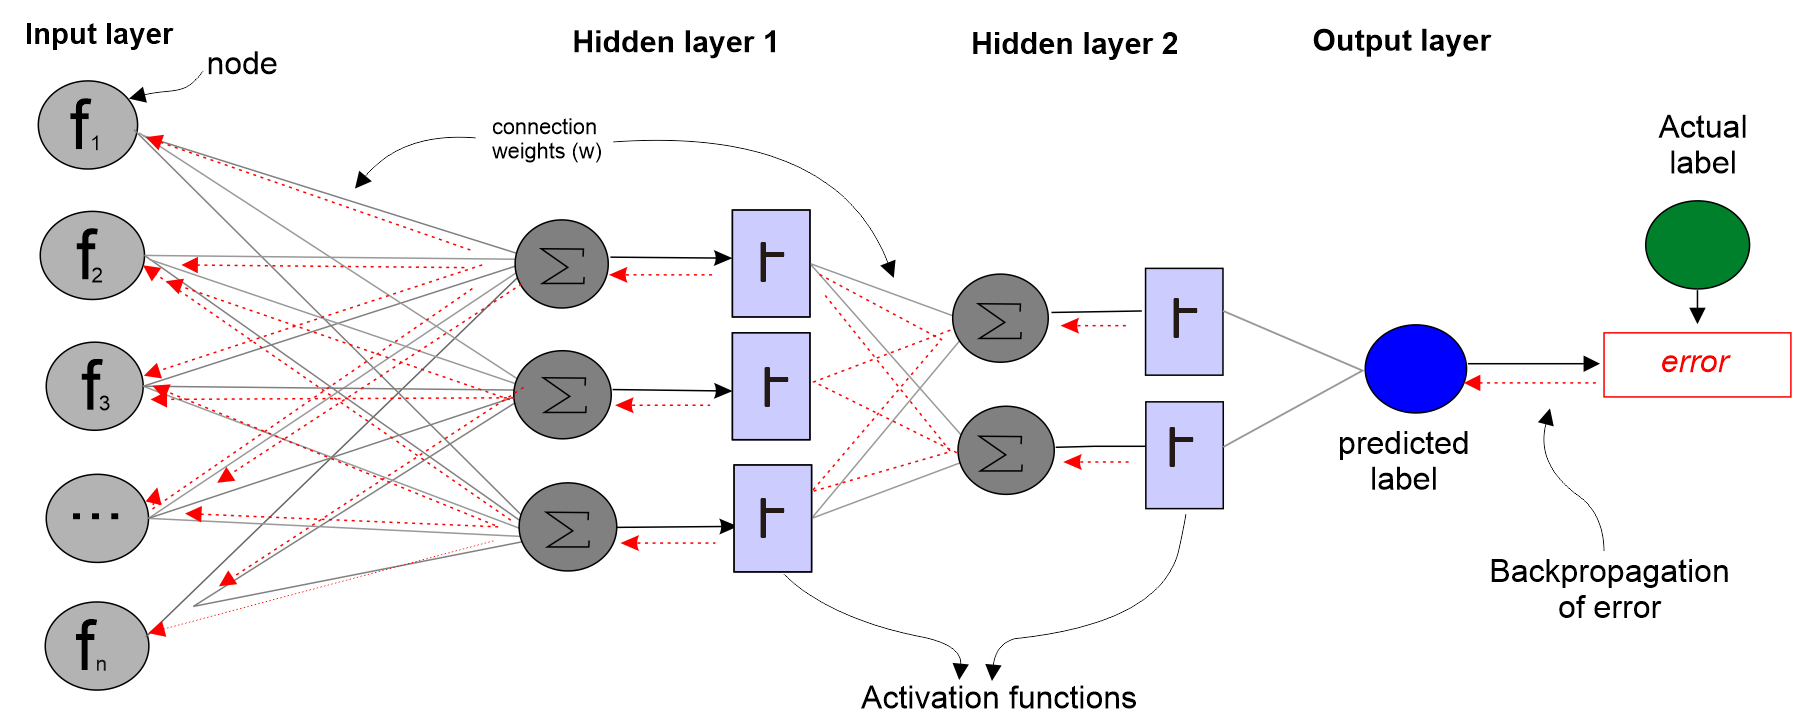
\includegraphics[width=0.9\textwidth,height=65mm]{images/ffnn_1.png}
    \caption{The architecture of a MLP with an input layer, 2 hidden layers, and an output layer}
    \label{fig:mlp_1}
\end{figure}

\hspace*{3.5mm} RBMs are the basic building blocks for DBNs. Unlike MLP, which is an FFNN that's trained in a supervised way, DBNs are trained in two phases: unsupervised pretraining and supervised fine-tuning. In unsupervised pretraining, layers are stacked in order and trained in a layer-wise manner with used unlabeled data. In supervised fine-tuning, an output classifier layer is stacked and the complete neural network is optimized by retraining with labeled data. One problem with MLP is that it often overfits the data, so it doesn't generalize well. To overcome this issue, DBN was proposed , which uses a greedy, layer-by-layer, pretraining algorithm and composed of a visible layer and multiple hidden unit layers. However, despite numerous successes, DBNs have been replaced with AEs. 

\subsection{Autoencoders}
\label{preli:AEs}
A regular AE consists of multi-layer dense networks called encoder and decoder, which is architecturally an MLP~\cite{karimDLTF2018}. AE also acts data compression technique where the compression and decompression functions are data-specific, lossy, and learned automatically from samples rather than human-crafted manual features~\cite{karimDLTF2018}. The encoder learns the representation of input $X$ in a compressed format in which the data is mapped and transformed into an embedding $Z$.  

\begin{figure}[h]
    \centering
    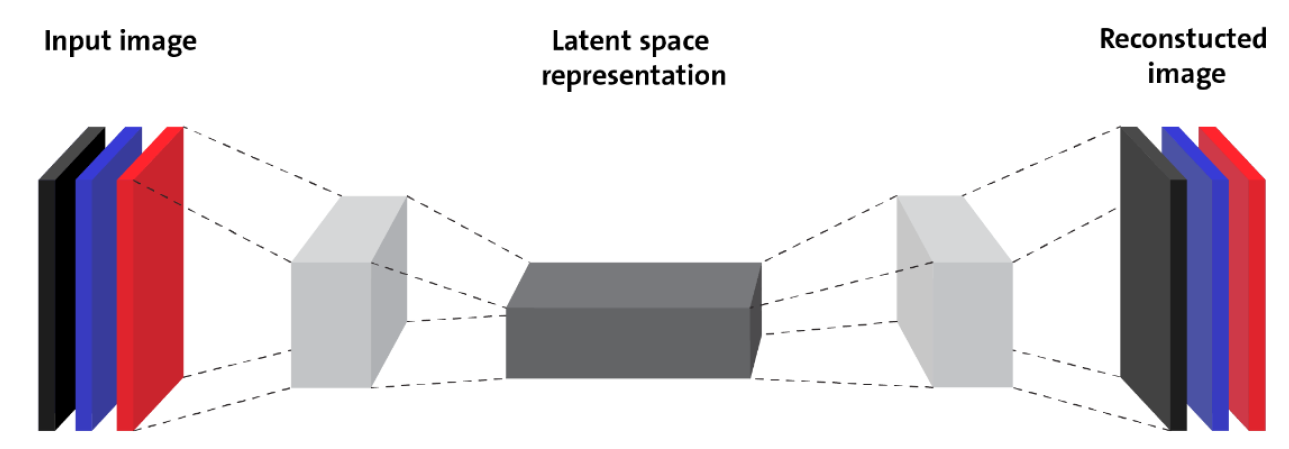
\includegraphics[width=0.55\textwidth,height=65mm]{images/ae.png}
    \caption{An unsupervised autoencoder as a network for latent feature learning~\cite{karimDLTF2018}}
    \label{fig:ae_theory1}
    \vspace{-2mm}
\end{figure}

%The decoder module of the AE network maps $Z$ to the reconstruction $X^{\prime}$~\cite{karimACCESS2019}, i.e., by approximating a function, $h_{W, b}(x) \approx x$, the decoder module to the identity function in order to output $\chi^{\wedge}$, which is similar original input x. 
\hspace*{3.5mm} Then the decoder tries to reconstruct $X$ from $Z$ by reducing the reconstruction loss between $X$ and its corresponding reconstruction $X^{\prime} \in \mathbb{R}^{D}$ such that useful information is not lost in the encoding phase~\cite{KarimIEEEAccess2019}.

\vspace{-2mm}
\begin{itemize}[noitemsep]
    \item \textbf{Encoder}: encodes the input into a latent-space representation using function $h = f(X)$.
    \item \textbf{Decoder}: reconstructs the input from the latent space representation using function $\tilde{x} = g(h)$. 
\end{itemize}
\vspace{-2mm}

Usually, reconstruction loss is the distance measure~($d_{AE}$) between input $x_i$ and network's output $f(x_i)$: 

\vspace{-2mm}
\begin{equation}
    L_{AE}=\text{$d_{AE}$}(x_i, f(x_i) = \sum_{i} ||x_{i}-f(x_i)||^{2}.
    \label{eq:Loss1}
\end{equation}

\hspace*{3.5mm} The identity function seems a particularly trivial function to be trying to learn, but by placing constraints on the network, such as by limiting the number of hidden units, we can discover interesting features of the data~\cite{karimDLTF2018}. Although used for learning representations from numeric data and LQ images, AE is mostly not suitable for 2D/3D finite and discrete signals or digital images~\cite{min2018survey}, primarily because of their weak RL capability. In \cref{sec:rep_learn}, we discuss different variants of autoencoders for the representation learning, which we will use in subsequent chapters. 

\subsection{Convolutional neural networks}
DNNs have no prior knowledge of how the pixels are organized because they do not know that nearby pixels are close. CNNs embed this prior knowledge using lower layers by using feature maps in small areas of the image, while the higher layers combine lower-level features into larger features. This setting works well with most of the natural images, giving CNN a decisive head start over DNNs~\cite{karimIoT2019}. CNNs have achieved much and have been widely adopted in computer vision, e.g., image recognition. The connection schemes in a CNN are significantly different compared to an MLP or DBN. A few of the convolutional~(conv) layers are connected in a cascade style. 

\begin{figure}[h]
    \centering
    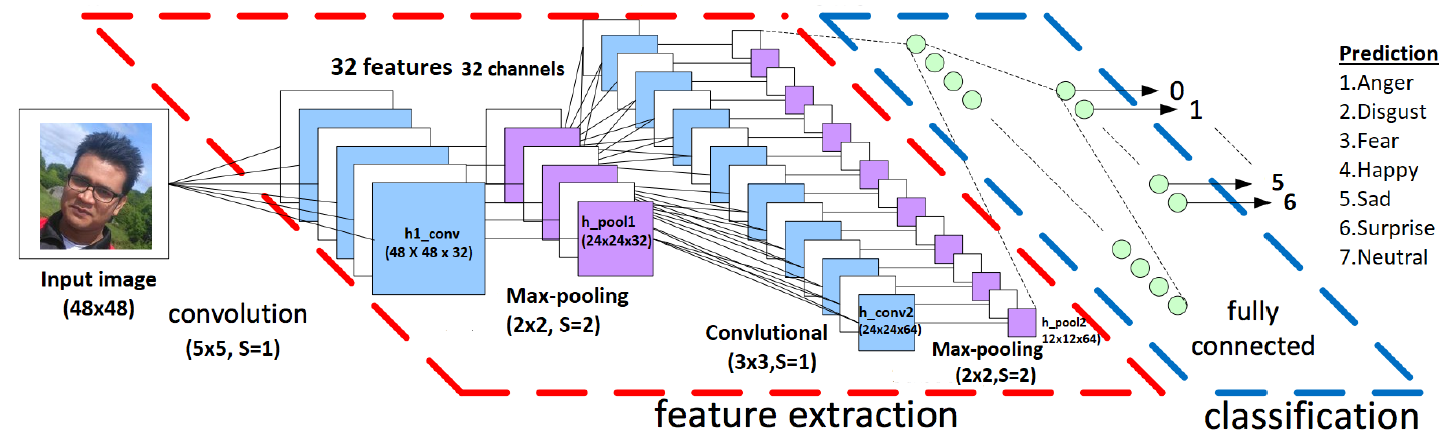
\includegraphics[width=0.9\textwidth,height=50mm]{images/cnn.png}
    \caption{A schematic architecture of a CNN used for facial recognition~\cite{karim2017predictive,zaccone2018deep}}
    \label{fig:cnn_theory1}
\end{figure}

\hspace*{3.5mm} The output from each conv layer is a set of objects, called feature maps generated by a single kernel filter. Then, the feature maps can be used to define a new input to the next layer. Each neuron in a CNN network produces an output followed by an activation threshold, which is proportional to the input and not bound. Each layer is backed up by an ReLU layer, a pooling layer, additional conv layers (+ReLU), and another pooling layer, which is followed by a fully connected layer~(FCL) and a softmax layer. The preceding diagram~(\cref{fig:cnn_theory1}) is a schematic architecture of a CNN used for facial recognition, which takes facial images as input and predicts emotions such as anger, disgust, fear, happy, and sad ~\cite{karimDLTF2018}.  
%A neuron can be active (or firing) if its output value is close to 1, or inactive if its output value is close to 0. However, for simplicity, we assume that the neurons are inactive most of the time. This argument is true as long as we are talking about the sigmoid activation function. However, if you are using the tanh function as an activation function, then a neuron is inactive when it outputs values close to -1.

\subsection{Recurrent neural networks}
Traditional neural networks instead ignore past events, as it is not possible for a neural network to use past scenes to classify current ones. In contrast to conventional neural networks, RNNs are networks with a loop that allows the information to be persistent in a neural network. The backpropagation time rolls out the RNN, creating a very deep feed-forward neural network. The impossibility of getting a long-term context from the RNN is due precisely to this phenomenon: if the gradient vanishes or explodes within a few layers, the network will not be able to learn high temporal distance relationships between the data. 

\begin{figure}[h]
    \centering
    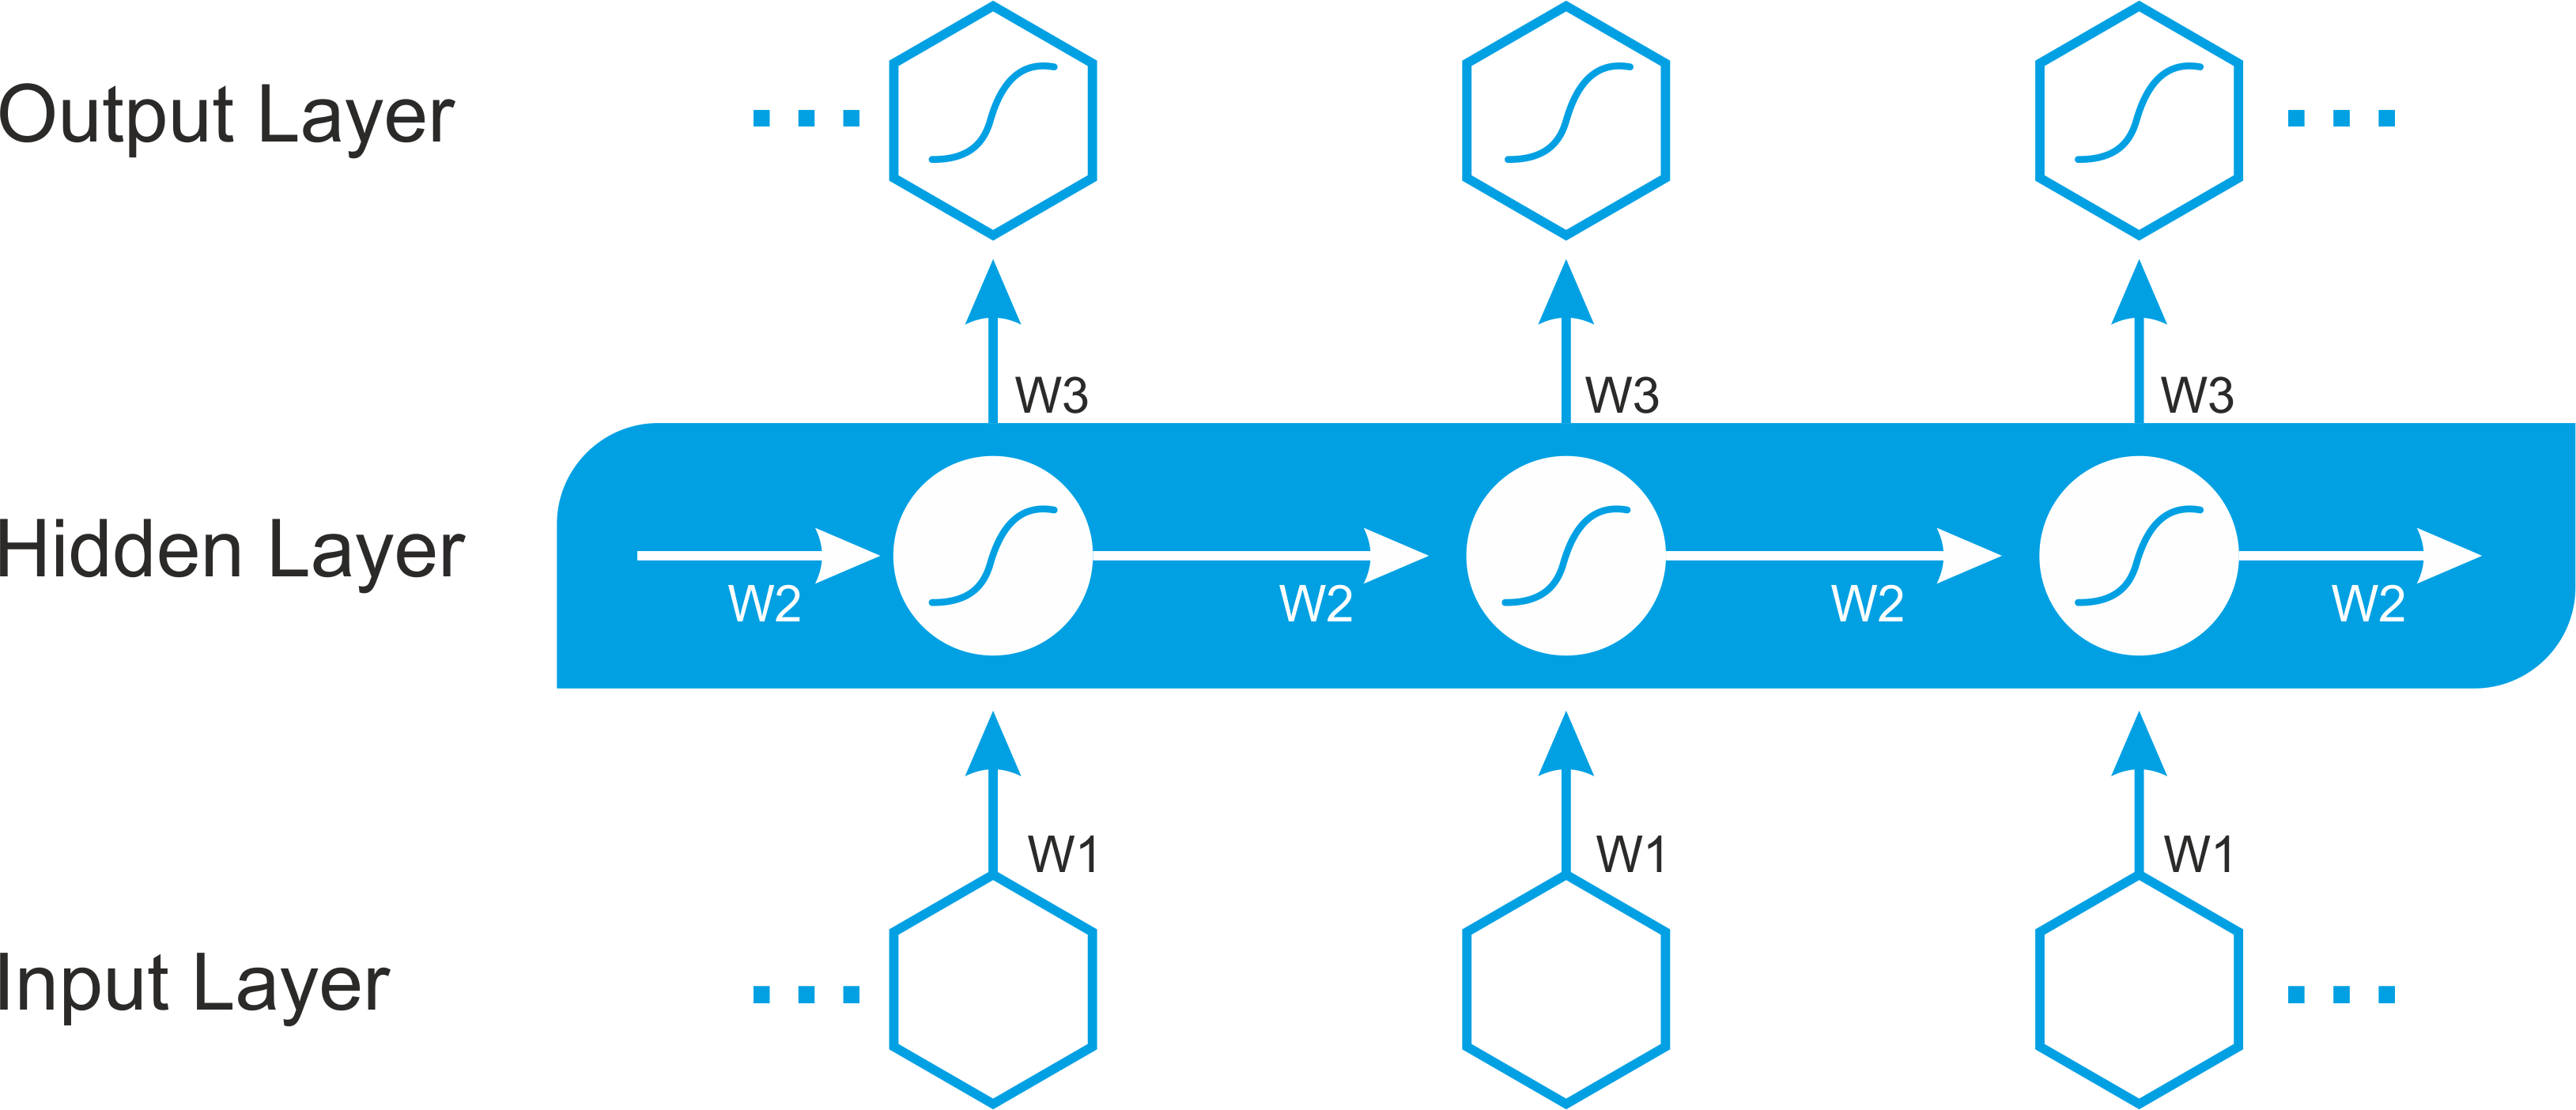
\includegraphics[width=0.7\textwidth,height=45mm]{images/B09698_06_4.png}
    \caption{In RNN all the weights in all the layers have to be learned with time~\cite{karimDLTF2018}}
    \label{fig:rnn_theory1}
    \vspace{-2mm}
\end{figure}

\hspace*{3.5mm} The preceding diagram~(\cref{fig:rnn_theory1}) is a schematic architecture of a RNN, where all the weights in all the layers have to be learned with time~\cite{karimDLTF2018}. However, the computed and back-propagated gradient tends to decrease~(or increase) at each instant of time and then, after a certain number of instants of time, the cost function tends to converge to zero (or explode to infinity). However, improved RNN variants such as LSTM, bi-directional LSTM, and GRU can combat the vanishing gradients and offers excellent results and performance. LSTM-based networks are ideal for the prediction and classification of temporal sequences and are replacing many traditional approaches to DL. As the name signifies, that short-term patterns are not forgotten in the long term. 

\subsection{Emergent architectures}
Many other emergent DL architectures have been suggested, such as Deep SpatioTemporal Neural Networks~(DST-NNs), and Multi-Dimensional Recurrent Neural Networks~(MD-RNNs). Nevertheless, there are a few more emerging networks, such as CapsNets - an improved version of a CNN, RNN for image recognition, and Generative Adversarial Networks~(GANs) for simple image generation. Apart from these, factorization machines for penalization and DL are also being used widely. 

\subsubsection{Residual neural networks}
Since there are sometimes millions and millions of hyperparameters and other practical aspects, it's really difficult to train deeper neural networks. To overcome this limitation, a residual learning framework is proposed~\cite{zagoruyko2016wide} to ease the training of networks that are substantially deeper than those used previously. They also explicitly reformulated the layers as learning residual functions with reference to the layer inputs, instead of learning non-referenced functions. This way, these residual networks are easier to optimize and can gain accuracy from considerably increased depth. The downside is that building a network by simply stacking residual blocks inevitably limits the optimization ability. %To overcome this limitation, Ke Zhang et al. also proposed using a multilevel residual network.

\subsubsection{Generative adversarial networks}
GANs architectures consist of two networks pitted against each other introduced by Ian Goodfellow et al.~\cite{GAN}. In GANs, two main components are the generator and discriminator. In a GAN architecture, a generator and a discriminator are pitted against each other—hence the name - adversarial~\cite{GAN}:

\vspace{-2mm}
\begin{itemize}[noitemsep]
    \item \textbf{Generator}: the generator tries to generate data samples out of a specific probability distribution and is very similar to the actual object.
    \item \textbf{Discriminator}: the discriminator will judge whether its input is coming from the original training set or from the generator part. 
\end{itemize}

\vspace{-2mm}
\begin{figure}[h]
    \centering
    \vspace{-3mm}
    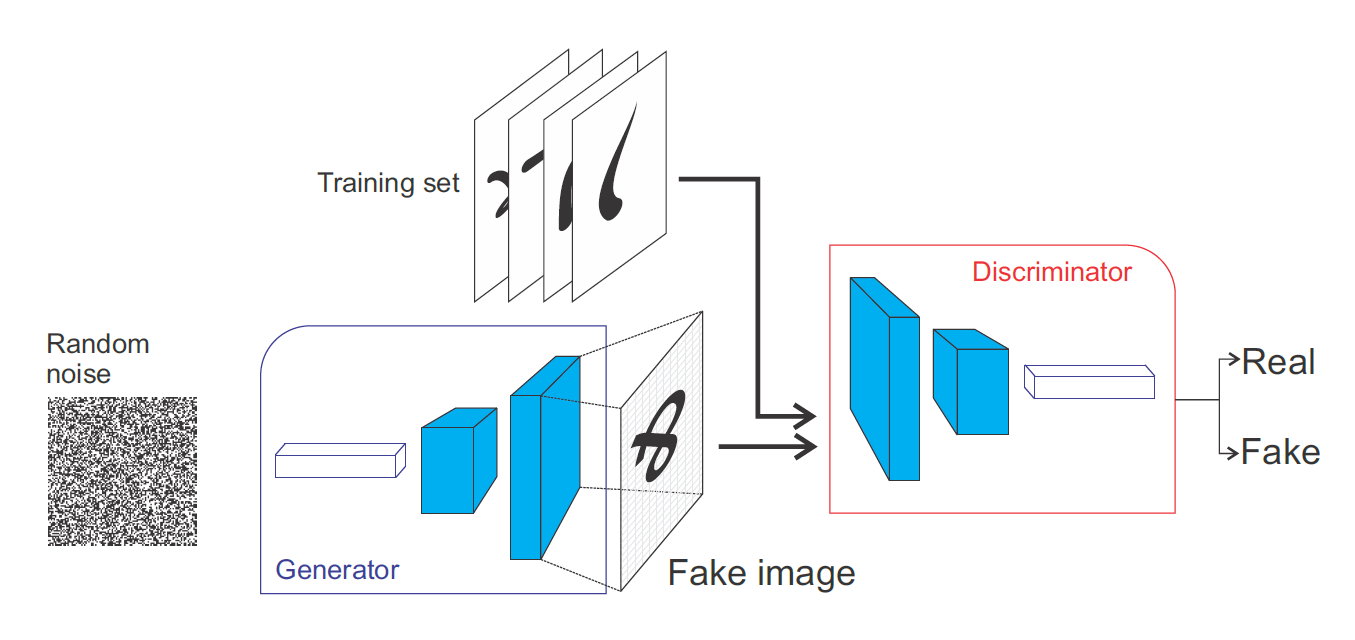
\includegraphics[width=0.75\textwidth,height=50mm]{images/gan.png}
    \caption{Schematic diagram of a simple GAN~\cite{karimDLTF2018}}
    \label{fig:gan}
    \vspace{-2mm}
\end{figure}

\hspace*{3.5mm} \Cref{fig:gan} shows a schematic diagram of a simple GAN. Many DL practitioners think that GANs were one of the most important advancements because GANs can be used to mimic any distribution of data, and, based on the data distribution, they can be taught to create robot artist/super-resolution images, text to image synthesis, speech. Facebook's AI research director, Yann LeCun, thinks GANs are the most interesting idea in the last 10 years of ML\footnote{See: Generative Adversarial Networks: What Are They and Why We Should Be Afraid, by Thomas Klimek, 2018}.

\subsubsection{Capsule networks}
In CNNs, each layer understands an image at a much more granular level through a slow receptive field or max pooling operations. If the images have rotation, tilt, or very different shapes or orientation, CNNs fail to extract such spatial information and show very poor performance at image processing tasks. Even the pooling operations in CNNs cannot be much help against such positional invariance. This issue in CNNs has led CapsNet~\cite{CapsNet}, where a capsule is a group of neurons whose activity vector represents the instantiating parameters of a specific type of entity, such as an object or an object part~\cite{CapsNet}.

\begin{figure}[h]
    \centering
    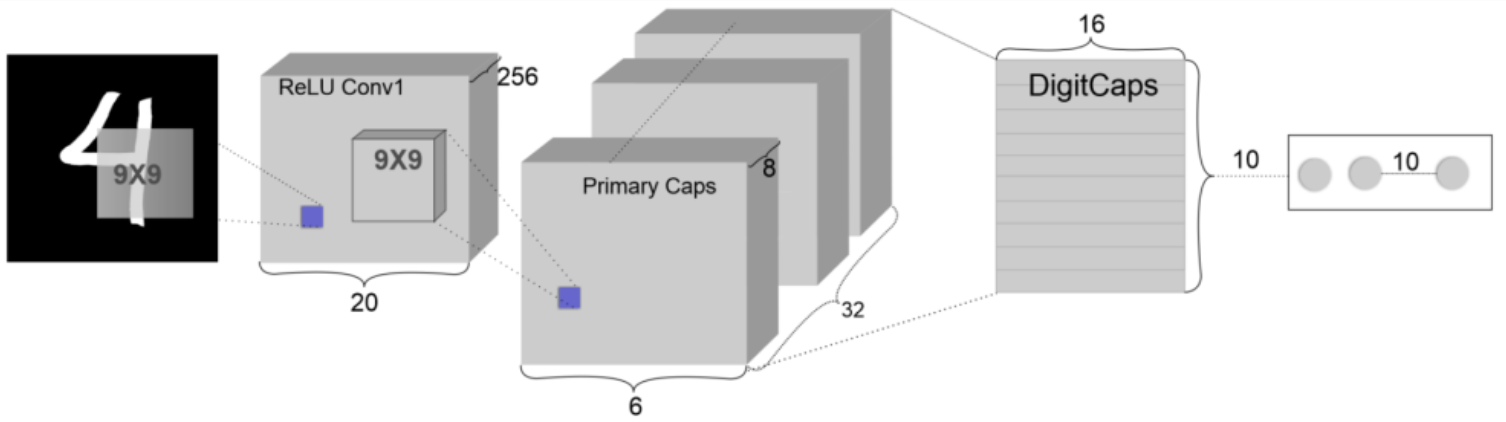
\includegraphics[width=0.9\textwidth,height=40mm]{images/capsnet.png}
    \caption{Schematic diagram of a simple three-layer CapsNet~\cite{karimDLTF2018}}
    \label{fig:capsnet}
\end{figure}

\hspace*{3.5mm} Unlike a regular DNN, where we keep on adding layers, in CapsNet, the idea is to add more layers inside a single layer, making the CapsNet a nested set of neural layers~\cite{CapsNet}. In CapsNet, the vector inputs and outputs of a capsule are computed using the routing algorithm used in physics, which iteratively transfers information and processes the self-consistent field~(SCF) procedure. \Cref{fig:capsnet} shows a schematic diagram of a simple three-layer CapsNet. The length of the activity vector of each capsule in the DigiCaps layer indicates the presence of an instance of each class, which is used to calculate the loss. 

\section{Representation Learning}
\label{sec:rep_learn} 
Representing raw data in a format that a ML model can work with has always been a big challenge in order to develop DSS~\cite{mmsurvey}. Images, audio samples, individual words, or a sentence features are often represented in vector or tensor formats, which is called representation learning~(RL). In this section, we discuss different RL techniques for both unimodal and multimodal datasets. 

\subsection{Learning representation from unimodal data}
While the development of unimodal representations has been extensively studied, there has been a shift from hand-designed for specific applications to data-driven~\cite{mmsurvey}. Subsequently, several ways by employing different neural network architectures have been proposed to improve the quality of the representation learning~\cite{min2018survey} from such datasets. In some early approaches, deep belief networks~(DBN) is employed as the feature extractor in which restricted Boltzmann machines~(RBM)~\cite{jaitly2011learning} formed the basic building block. 

\hspace*{3.5mm} Each successive layer of a deep RBM is stacked together to represent the data at a higher level of abstraction. One advantage of RBM for RL is it does not need much labeled data for the training. Being the graphical models, the representation of data is probabilistic. Besides, the scale invariant feature transform was often used in imaging, which is gradually shifted to CNN with which most visual descriptions are learned from data. However, despite numerous successes, DBN has gradually been replaced with AE. 

\subsubsection{CAE}
Since a vanilla AE is not suitable for handling data with spatial invariance~(e.g., HQ images), they are incapable of preserving spatial relationships between pixels in an object. However, CNN can be a better feature extractor as it can preserve local structure in which output from the deepest convolutional~(conv) layer can be extracted as LF. In contrast, instead of manually engineered conv filters, conv and pooling layers can be added to construct a CAE, where each layer consists of an encoder~(that performs convolution and pooling operations), and a decoder~(to perform unpooling and deconvolution operations), and a conv layer of the encoder calculates the $j^{th}$ feature map as follows~\cite{alirezaie2019semantic}:

\begin{equation}
    h^{j}=\sigma\left(x_{i} * W_{ij}^{j}+b^{j}\right),
\end{equation}

where $x_i$ is the input sample, $W_{ij}^{j}$ is the $j^{th}$ filter from input channel $i$ and filter $j$, $b^j$ is the bias for the $j^{th}$ filter, i.e., single bias per latent map~(one bias per GV would introduce many degrees of freedom), $\sigma$ is an activation function~(i.e., rectified linear unit~(ReLu)), and $*$ denotes the conv operation. To obtain translation-invariant representations, max-pooling is performed by downsampling conv layer's output and taking the maximum value in each $m \times n$ non-overlapping sub-region~\cite{alirezaie2019semantic}. In the decoding phase, unpooling and deconvolution operations performed to preserve the positional-invariance information during the pooling operations. Then the deconvolution operation is performed to reconstruct $x_i$ as follows~\cite{alirezaie2019semantic}:

\begin{equation}
   x_i = \sigma\left(o^{j} * W_{oj}^{j}+c^{j}\right),
\end{equation}

where $o^j$ is $j^{th}$ feature map and $W_{oj}^{j}$ is $j^{th}$ filter of unpooling layer $o$; $j$ and $c^j$ are filter and bias of $j^{th}$ output layer, respectively. Compared to CNN~(e.g., DBC, CEN, DCEN, and DEPICT), CAE learns optimal filters and minimize the reconstruction loss, which results in more abstract features from the encoder~(e.g., pixel-level features from images) that help to stabilize training and network converges faster, avoid corruption in feature space, and improve the CQ~\cite{guo2017deep}. Besides, AAE, VAE, or LSTM-AE can be constructed in different scenarios~(e.g., imaging, sequence) for the RL. 

\begin{sidewaystable*}
   \caption{Comparison of autoencoders-based representation learning approaches~\cite{karimBIB2019}} 
   \label{tab:fe}
   %\scriptsize % text size of table content
   \centering % center the table
   \begin{tabular}{p{3.5cm}|p{10.3cm}|p{10cm}}
    \hline
   \textbf{Feature extractor} & \textbf{Advantages} & \textbf{Disadvantages}\\ 
   \midrule
    \textbf{AE} & One of the simplest and MLP-based auto-encoding techniques. It learns hidden features to encode and decode the data without considering the probability distribution of the input samples. Hence it is easy to implement and extract features from the encoder component. & AEs have a huge number of hyperparameters, which is why it is tricky to optimize and balancing between clustering and non-clustering losses. Since it learns the hidden representation discriminatively to encode and decode the data blindly using a shallow network architecture. A fundamental problem with an AE is with the LF it embeds their inputs to and where their encoded vectors lie), may not be continuous and may allow easy interpolation. Consequently, CQ would be poor in the case of bioimaging and biological sequence data. Although the computational complexity depends on the clustering loss, it requires many iterations to optimize a large number of hyperparameters.\\\hline
    \textbf{DBN} & A simple generative model based on RBM, which has very rich mathematical and conceptual justification in its structure as well as its training algorithms. Works moderately well even in a limited labeled data set because it can be pre-trained in an unsupervised way, and the pre-training weights can be reused for a supervised learning task. & DBN-based RL has a risk of obtaining a corrupted LF space if the RBM pretraining loss goes out-of-bounds. Further, to avoid overfitting, it typically requires many samples to train well.\\\hline
    \textbf{CNN} & Has a straightforward graceful objective hence can be extended to large-scale clustering tasks. Deep and quality features can easily be extracted for numerous bioinformatics use cases, e.g., bioimaging, text (i.e., sequence) clustering, and genomics. It has a fewer number of hyperparameters than a regular AE or VAE, which makes it easier to optimize the overall network. & Since there is a risk of obtaining a corrupted LF space, a well-defined clustering loss is required to balance between clustering and non-clustering losses, which is tricky. To avoid overfitting, CNN typically requires many samples to get trained well.\\\hline
    \textbf{CAE} & Has straightforward graceful objective hence can be extended to large-scale clustering tasks. Deep and quality features can be easily extracted for bioimaging and text clustering. Further, since in CAEs, weights are shared among all locations in the input, preserving locality, and reducing the number of parameters than regular AEs, VAEs, and CNNs~\cite{lintas2017artificial}. & Since there is a risk of obtaining a corrupted LF space, a well-defined clustering loss is required to balance between clustering and non-clustering losses, which is tricky. Similar to CNN, CAE also requires many samples to be trained well to avoid overfitting.\\\hline
    \textbf{VAE} & Capable to generate artificial samples, which makes it suitable for bioinformatics use cases with limited labeled or unlabeled samples. Particularly suitable for numeric and genomic data. Besides, it has a decent theoretical guarantee and mathematical interpretation. & The computational complexity is very high, hence requires many iterations to optimize numerous hyperparameters. Exhibits poor clustering in the case of HQ bioimaging. \\\hline
    \textbf{AAE} & Capable to generate artificial samples, which makes it suitable for bioinformatics use cases with limited labeled or unlabeled samples. Particularly suitable for numeric and genomic data. Besides, the flexible nature of GAN and its variants can be used to disentangle both discrete and continuous latent factors. Hence, it can scale to complex datasets. & Since AAE's optimizing objective comprises several losses~(i.e., reconstruction loss, GMM likelihood, and adversarial objective), computation complexity is very high and hard to converge. \\\hline
   \end{tabular}
\end{sidewaystable*}

\subsubsection{Variational autoencoders} 
Generative variants of AE called Variational autoencoders~(VAE) are used in literature in combination with a mixture of Gaussian. VAE enforces the latent code of AE to follow a predefined distribution, which combines variational Bayesian methods and increases the flexibility of the base network. Architecturally, VAE is different compared to AE or CAE and deeply rooted in the methods of variational Bayesian and graphical models, where the input is into distribution, as shown in \cref{fig:vae}. This distribution, say $p_{\theta}$, is parameterized by $\theta$, where $p_{\theta}(\mathbf{z})$ is the prior, $p_{\theta}(\mathbf{x} | \mathbf{z})$ is the likelihood, and $p_{\theta}(\mathbf{z}|\mathbf{x})$ is the posterior given that the real parameter $\theta^*$ is known for the distribution. 

\begin{figure*}[h]
	\centering
	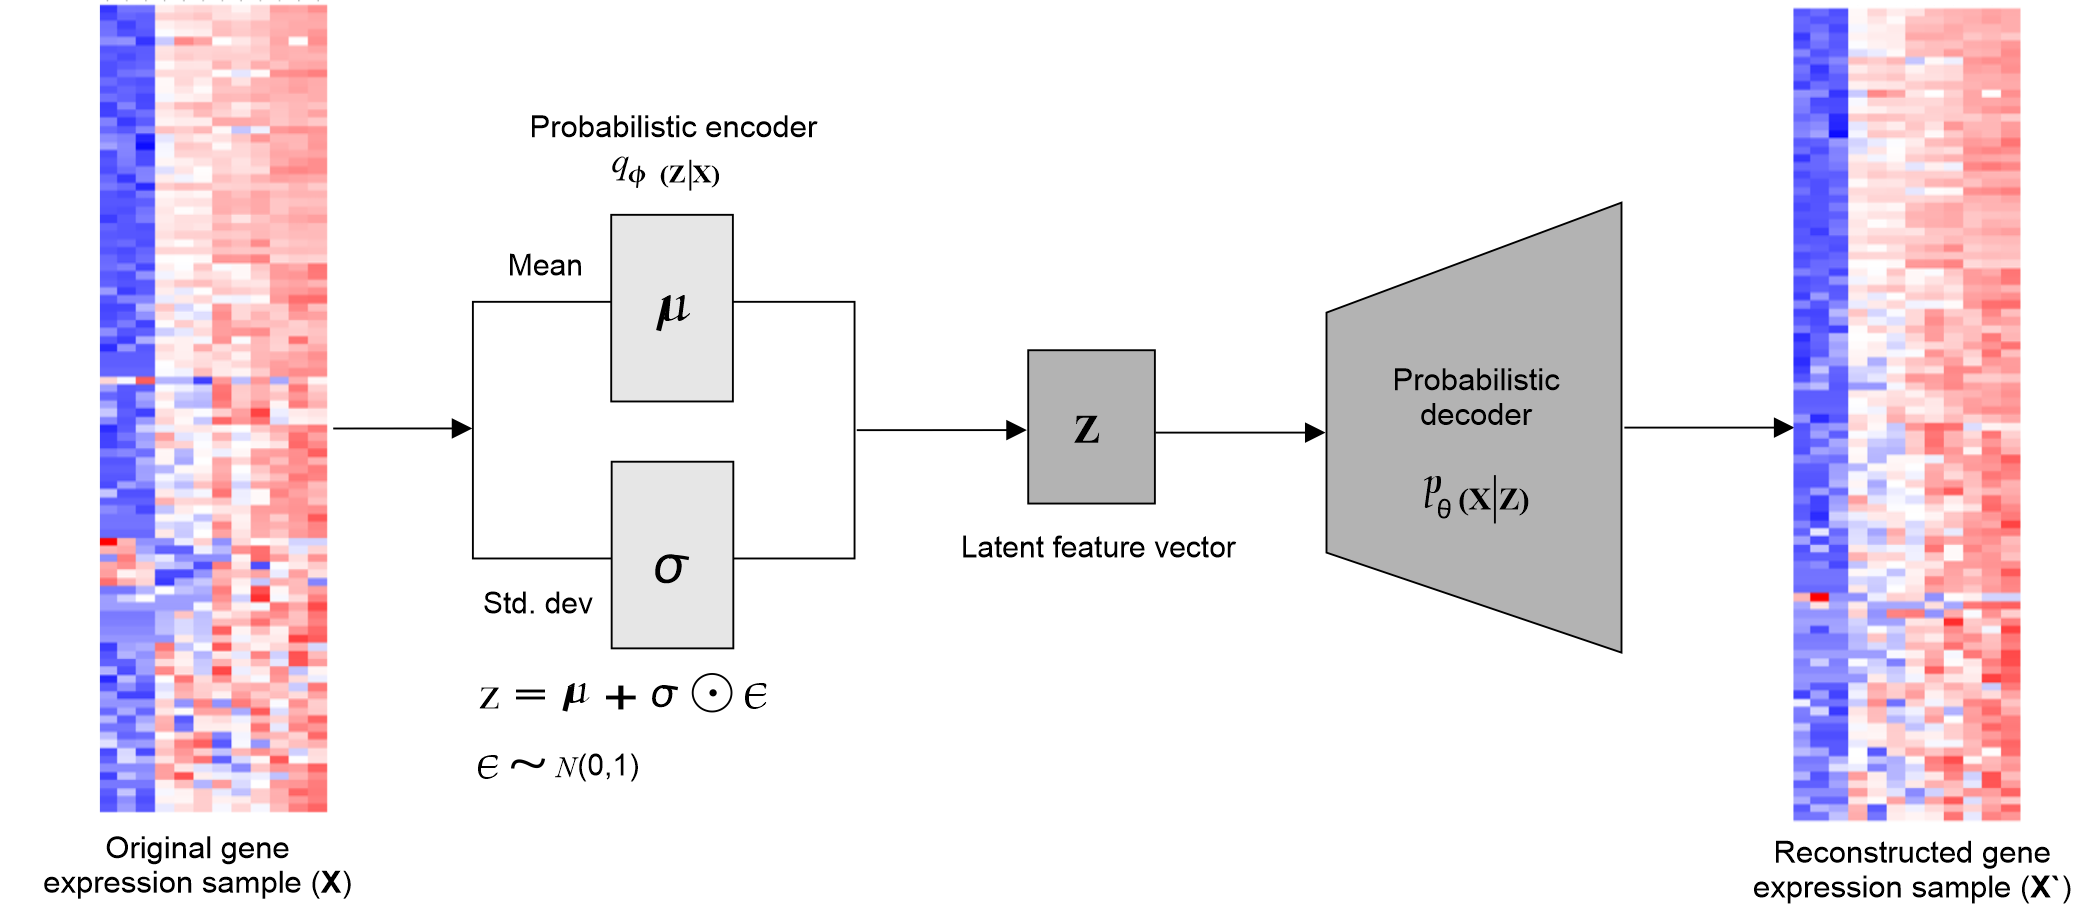
\includegraphics[width=\textwidth,height=70mm]{images/vae.png}	
	\caption{Schematic representation of a VAE used for clustering GE data, where an individual GE sample is fed into the model for learning representation~\cite{karimBIB2019}.}	
	\label{fig:vae}
	\vspace{-4mm} 
\end{figure*}

\hspace*{3.5mm} To generate a sample similar to a real data point $\mathbf{x}^{(i)}$: i) first, $\mathbf{z}^{(i)}$ can be sampled from a prior distribution $p_{\theta^{*}}(\mathbf{z})$, ii) then,  $\mathbf{x}^{(i)}$ can be generated from the conditional distribution $p_{\theta^{*}}\left(\mathbf{x} | \mathbf{z}=\mathbf{z}^{(i)}\right)$, $\theta^{*}$ is the optimal parameter that maximizes the probability of generating real data samples~\cite{VADE}:

\begin{equation}
    \theta^{*}=\arg \max _{\theta} \sum_{i=1}^{n} \log p_{\theta}\left(\mathbf{x}^{(i)}\right).
\end{equation}

\begin{equation}
    p_{\theta}\left(\mathbf{x}^{(i)}\right)=\int p_{\theta}\left(\mathbf{x}^{(i)} | \mathbf{z}\right) p_{\theta}(\mathbf{z}) d \mathbf{z}.
    \label{eq:data}
\end{equation}

\hspace*{3.5mm} The data generation process involving the encoding vector can be expressed in \cref{eq:data}~\cite{VADE}. Eventually, VAE consists of a probabilistic encoder as an approximation function $q_{\theta}(\mathbf{z} | \mathbf{x})$~(which is similar to $g_{\phi}(\mathbf{z} | \mathbf{x})$) and a generative probabilistic decoder as the conditional probability $p_{\theta}(\mathbf{x}|\mathbf{z})$~(which is similar to the decoder $f_{\theta}(\mathbf{x}|\mathbf{z})$). In variational inference, objective is to maximize the variational evidence lower bound (ELBO) by maximizing the lower bound (based on the fact that KL divergence is always non-negative, hence $-L_{vae}$ is the lower bound of $\log p_{\theta}(\mathbf{x})$) as follows~\cite{VADE}: 

\begin{equation}
    -L_{vae}=\log p_{\theta}(\mathbf{x})-L_{\mathrm{KLD}}\left(q_{\phi}(\mathbf{z}|\mathbf{x}) \| p_{\theta}(\mathbf{z}|\mathbf{x})\right) \leq \log p_{\theta}(\mathbf{x}). 
    \label{eq:lvae}
\end{equation}

\hspace*{3.5mm} VAE and its variants like LSTM-VAE~\cite{park2018multimodal}) are widely used across use cases,e.g., anomaly detection in which anomalous or outliers can be identified based on the reconstruction probability~(RP)~\cite{an2015variational}. RP is a probabilistic measure that takes into account the variability of the distribution of variables as: i) it has a theoretical background, and ii) more principled and objective anomaly score than the reconstruction loss. 

\subsubsection{LSTM-AE}
VAE or CAE are not the best options for handling sequence or time-series data, e.g., length of the input sequence in case of text clustering may vary while the network requires fixed-length inputs. Further, the temporal ordering of the observations makes the feature extraction difficult. Hence, regular AEs will fail to generate a sample sequence for a given input distribution in generative mode, whereas LSTM-AE can handle variable lengths as the encoder learns fixed-length vector representation of the input~\cite{KarimNCCA2019,karim2019drug}. Given $X$ = $\{\mathbf{x}^{(1)},\mathbf{x}^{(2)}, ..., \mathbf{L}^{(1)}\}$ a input sequence, $\mathbf{h}_E^{(i)} \in {R}^c$ is encoder's hidden state at time $t_i$ for each $i \in \{1,2,...,L\}$, and $c$ is the number of LSTM units~\cite{LSTM_Autoencoder}. The encoder and decoder are jointly trained to reconstruct the original vector in reverse order by minimizing the following objective~\cite{zhu2018hidden}:  

\begin{figure*}[h]
	\centering
	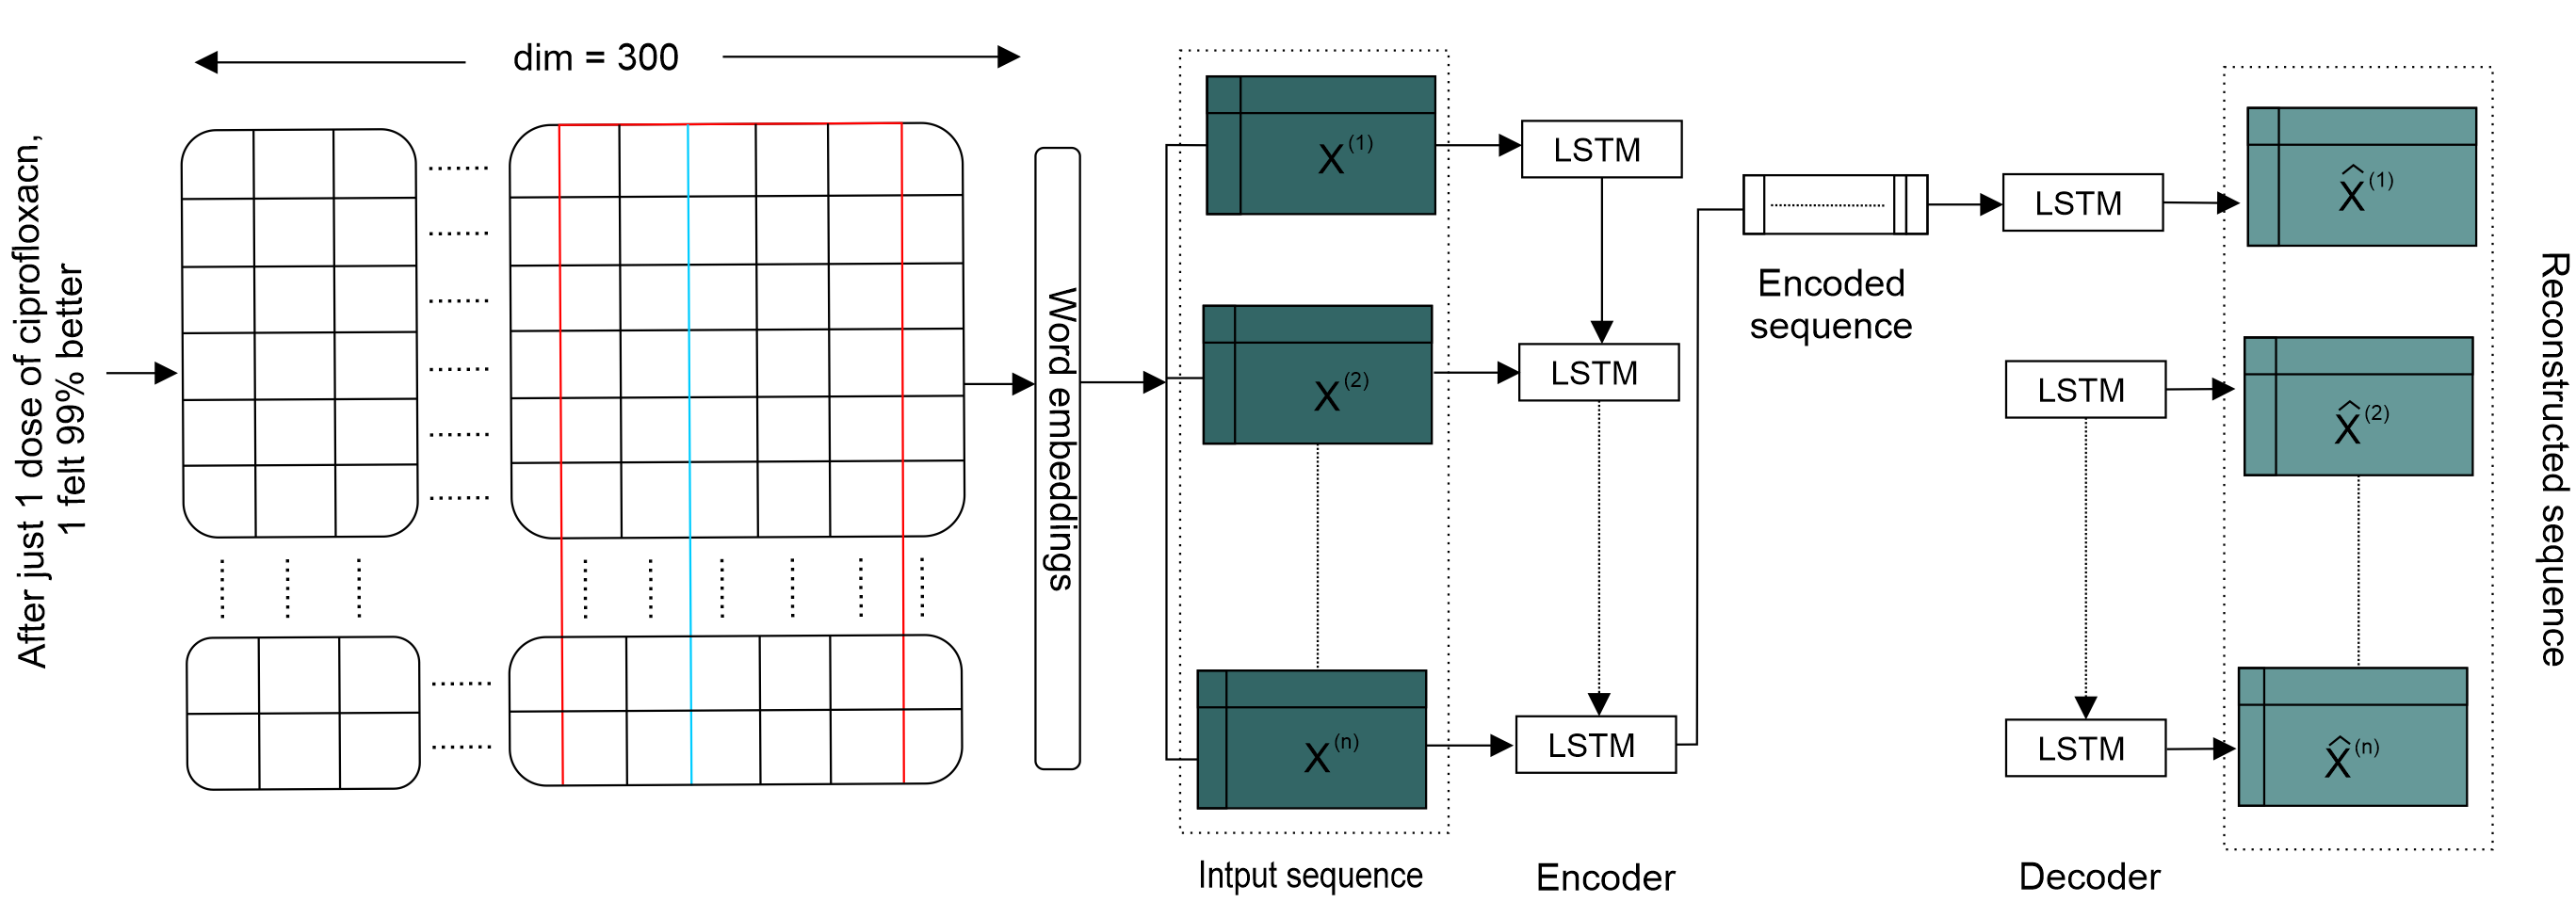
\includegraphics[width=\textwidth,height=70mm]{images/lstm_ae_v2.PNG}
    \caption{Schematic representation of the LSTM-AE, used for biomedical text clustering, where individual drug review texts are embedded using word2vec before feeding as a sequence~\cite{karimBIB2019}}	
	\label{fig:lstm_ae}
	\vspace{-2mm} 
\end{figure*}

\begin{equation}
    \sum_{X \in S_n}\sum_{i=1}^{L}\|\mathbf{x}^{(i)}-\mathbf{x}'^{(i)}\|^2
    \label{eq:obj}
\end{equation}

where $S_n$ is set of training sequences. The final state $\mathbf{h}_E^{(L)}$ of the encoder is used as the initial state for the decoder. The decoder uses $\mathbf{x}^{(i)}$ as input to obtain state $\mathbf{h}_D^{(i-1)}$ and predict $\mathbf{x'}^{(i-1)}$ corresponding to target $\mathbf{x}^{(i-1)}$~\cite{LSTM_Autoencoder} as shown in \cref{fig:lstm_ae}.  

\subsubsection{Adversarial autoencoders} 
In more recent approaches, adversarial autoencoders~(AAE) is employed in which the adversarial training procedure is followed to match the aggregated posterior of the latent representation with the prior distribution. AAE can be used to generate artificial samples with a limited number of labeled or unlabeled~(i.e., numeric or genomic) data, where the flexible nature of GAN can be utilized to extract discrete and continuous LF from large-scale data~\cite{min2018survey}. In particular, information maximizing generative adversarial network~(aka. InfoGAN)~\cite{chen2016infogan} is used for optimizing the mutual information between a fixed small subset of the GAN's noise variables and the observation~\cite{mcdaid2011normalized}, assuming: i) computation complexity is not a prime concern, ii) appropriate hyperparameters can be found. 

%\paragraph{\textbf{Sparse AE:}}  Besides, restrictions can be imposed to enforce the encoder to extract most salient features, e.g., sparsity constraint to obtain a sparse representation~\cite{min2018survey}. 
\subsubsection{Stacked autoencoders} 
The input can be denoised and passed through by stacking autoencoders~(SAE), e.g., where the input corruption is used only for the initial denoising. Once the mapping function $f_{\theta}$ is learned, the uncorrupted input from the previous layers are reused in the subsequent layers, e.g., then the weights of the network can be initialized with SDAE, where each layer is a DAE trained to reconstruct previous layer's output after random corruption~(i.e., DAE). SDAE can be considered a 2-layer network formulated as follows~\cite{xie2016unsupervised}:

\vspace{-6mm}
\begin{align}
    \begin{aligned}
        \tilde{x} & \sim d \text {ropout }(x) \\
        h &=g_{1}\left(W_{1} \tilde{x}+b_{1}\right) \\
        \tilde{h} & \sim d r o p o u t(h) \\
        y=& g_{2}\left(W_{2} \tilde{h}+b_{2}\right)
    \end{aligned}
\end{align}

\noindent where $dropout(.)$ is the dropout operation~\cite{srivastava2014dropout}, $g_1$ and $g_2$ are activation functions for encoding and decoding layer respectively, and $\theta$=$\lbrace{W_1, b_1, W_2, b_2}\rbrace$ are model hyperparameters~\cite{xie2016unsupervised}. Then greedy layer-wise training~(GLW) is performed by minimizing the least-squares loss $||x-y||^{2}_{2}$, i.e., after training one layer, output $h$ is used as the input to the next layer and so on. In such a scenario, ReLU activation function is used in all encoder and decoder pairs, except for $g_2$~(first pair) and $g_1$~(last pair). Once the GLW training is finished, all the encoder and decoder layers are concatenated in reverse layer-wise training order, by forming a deep AE and fine-tuned to minimize the reconstruction loss. During the GLW pre-training, each layer is pretrained for a relatively higher number of iterations with a dropout. The result is a multilayer deep AE with a bottleneck-coding layer in the middle. Based on a similar principle, other types of AE can be stacked to form such a deep AE architecture. 

\subsection{Learning representation from multimodal data}
A multimodal representation is a representation of data using information from multiple such entities~\cite{mmsurvey}. The ability to represent multimodal data in an efficient way is forms the backbone of any predictive model. However, how to combine different types of data from heterogeneous sources, how to deal with different levels of noise and artifacts, and how to deal with missing data are few challenges in the multimodal RL. To develop a DSS, we might need to represent one or multiple types of data, e.g., genomics, proteomics, or imaging data need to feed into the neural networks. \\

\vspace{-2mm}
\begin{tcolorbox}[colback=white!3!white,colframe=gray!120!black,title=\faBook~Input modality]
    %INFO: \faBook \\
    \scriptsize{
        \textbf{Input modality:} a decision support systems, which provides decision (e.g., clinical) relies on different types of data and in terms of dataset is characterized as multimodal. The term `modality' refers to the way in which we experience a real-life events that includes multiple such modalities~\cite{mmsurvey}.
        }
\end{tcolorbox}

\begin{figure*}[htp!]
	\centering
	\begin{subfigure}{.48\linewidth}
		\centering
		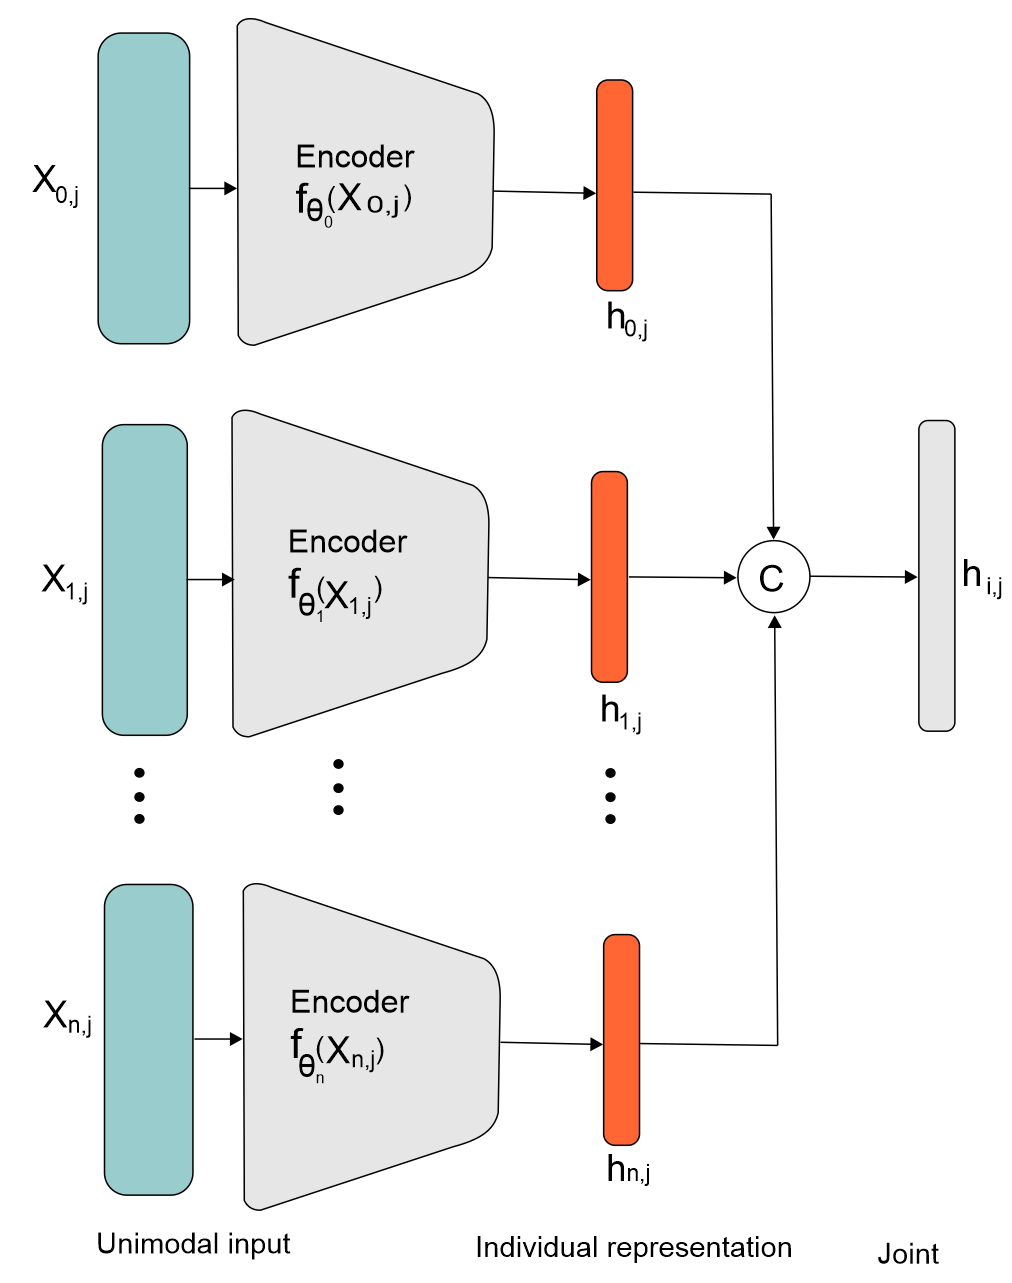
\includegraphics[width=0.95\linewidth,height=70mm]{images/rl_1.png}
		\caption{Latent representation concatenation}
        \label{fig:lrc_1}
	\end{subfigure}
	\begin{subfigure}{0.48\linewidth}
		\centering
		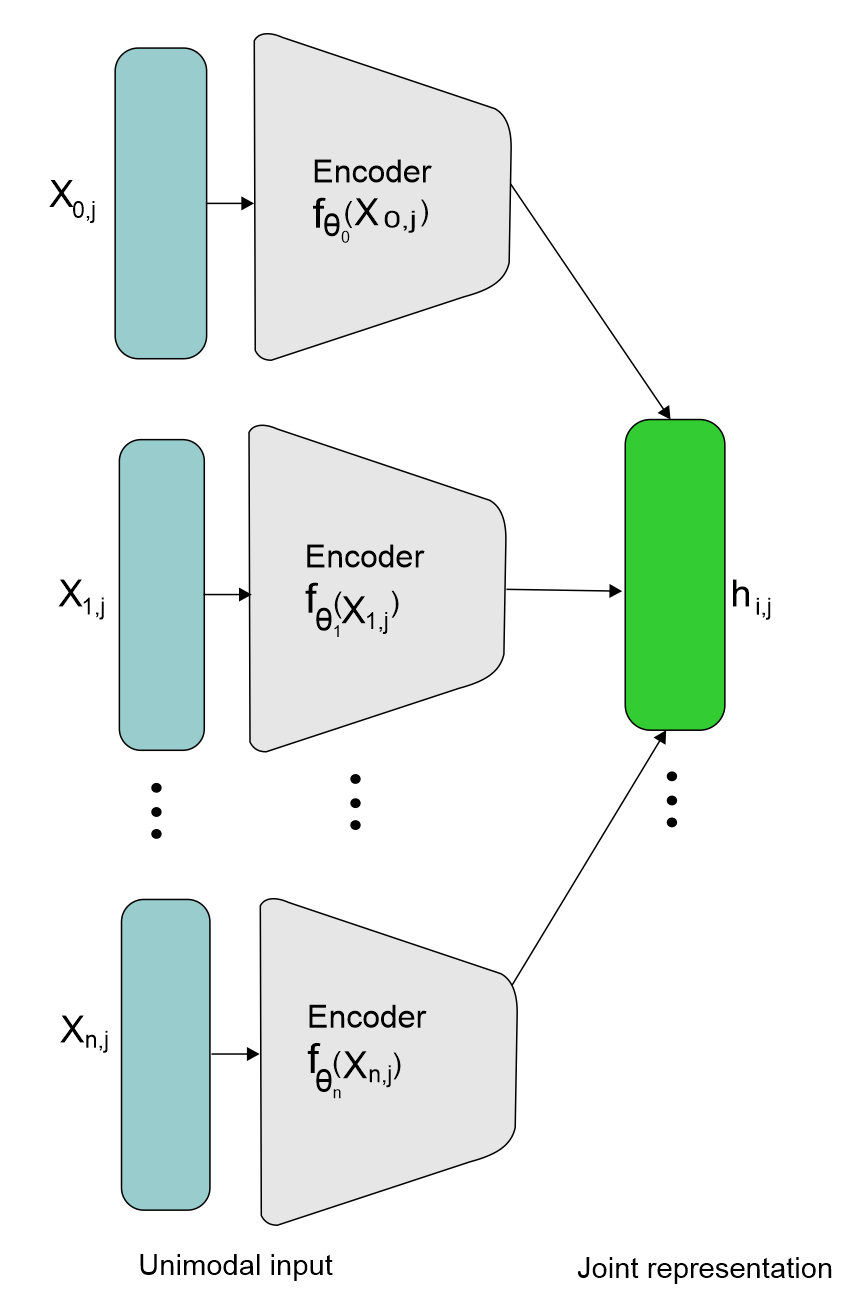
\includegraphics[width=0.95\linewidth,height=70mm]{images/shared.png}
		\caption{Shared latent representation}
        \label{fig:slr_1}
	\end{subfigure}
	\caption{Fusion architectures in multimodal representation learning (only encoder module is shown)} 
	\label{fig:mm_rL_example}
\end{figure*}

\hspace*{3.5mm} Although several works have focused on unimodal RL, recent approaches are more focused on multimodal representations from different types of data involving simple or shared concatenation of unimodal ones~\cite{mmsurvey}. \Cref{fig:mm_rL_example} shows two fusion architectures in multimodal RL. The latent representation concatenation architecture is depicted in \cref{fig:lrc_1} consists of learning simultaneously a single latent representation from each modality. In the subsequent chapters, we'll show how to use the concatenation of all the modality-specific latent representations to train a classifier. 

\section{Model Ensemble Methods}
The ensemble modelling is based on a principle in which weak learners is grouped together to form one strong learner. First, multiple models are trained, each with the objective to predict or classify a set of results. By using ensemble methods, the stability of the final model can be increased by reducing the errors. In particular, by combining many models, mostly the variance error can be reduced. For example, by maximum voting from a panel of independent radiologists, we get the final prediction fair and trustworthy than a single radiologist. 

\begin{figure*}[htp!]
	\centering
	\begin{subfigure}{.48\linewidth}
		\centering
		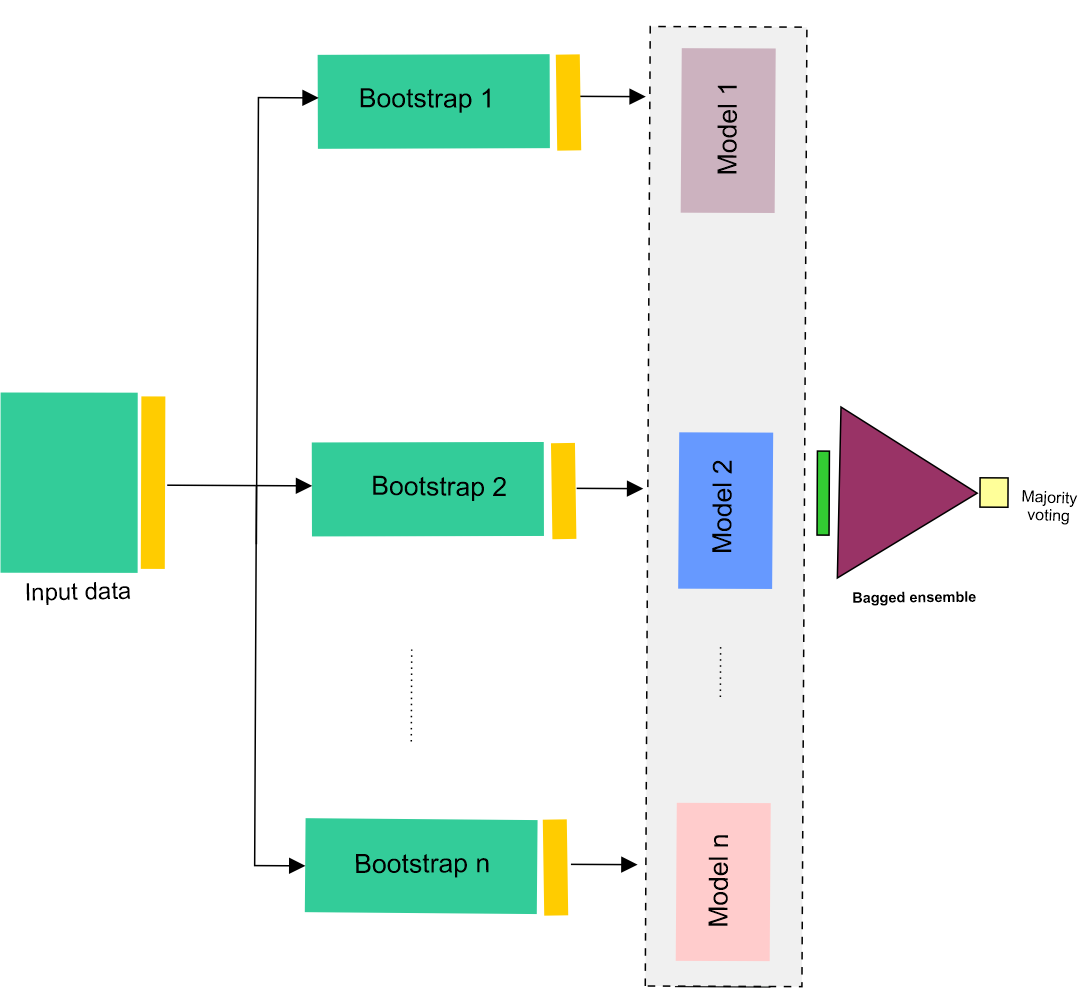
\includegraphics[width=\linewidth,height=65mm]{images/bagging.png}
		\caption{Bagging}
        \label{fig:bagging}
	\end{subfigure}
	\hspace{2mm}
	\begin{subfigure}{0.48\linewidth}
		\centering
		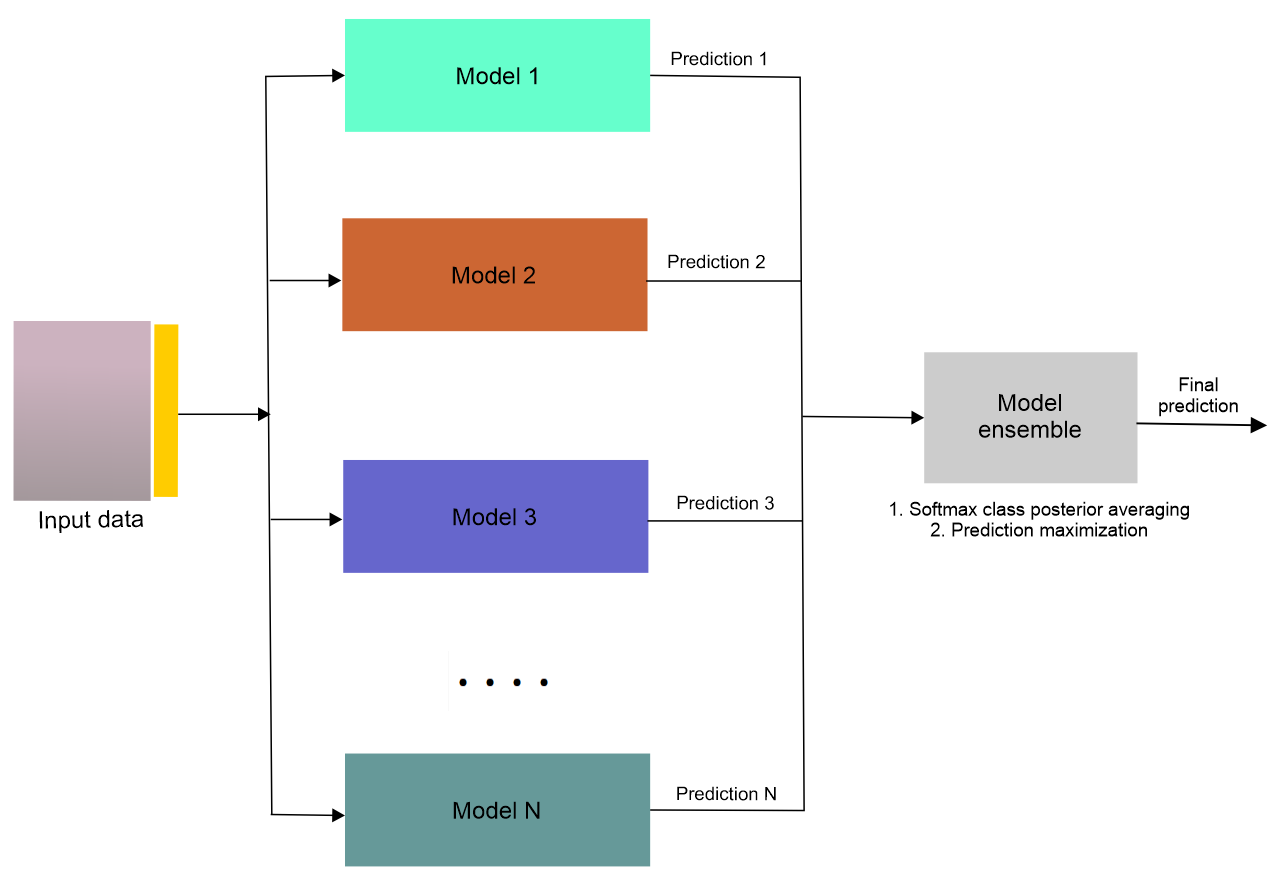
\includegraphics[width=\linewidth,height=65mm]{images/stacking.png}
		\caption{Stacking}
        \label{fig:stacking}
	\end{subfigure}
	\caption{Bagging vs. stacking: a) each model is individually trained and the predictions are voted upon, b) multiple weak learners are summed upon} 
	\label{fig:bagging_and_stacking}
	\vspace{-2mm}
\end{figure*}

\hspace*{3.5mm} In short, the model ensemble technique helps to achieve improved performance of a model compared to the predictions from a single model by reducing the generalization error~\cite{karimACCA2019}. Technically, bagging~(refer to \cref{fig:bagging}), boosting, and stacking~(refer to \cref{fig:stacking}) are three main concepts can be employed to create an ensemble method by reducing the variance, noise, and bias: \\

\vspace{-2mm}
\begin{tcolorbox}[colback=white!3!white,colframe=gray!120!black,title=\faBook~Ensemble concepts]
    \scriptsize{
        \textbf{Bagging:} is the combination of bootstrapping and aggregating the scores over many samples in order to decrease the model’s variance. Bootstrapping is a very well-known method that helps decrease model variance by reducing overfitting and resampling data from the training set with the same cardinality as the original set. Bagging is an effective method when you have limited data. \\
        \textbf{Boosting:} is adding additional models to the overall ensemble model sequentially to decrease model’s bias. \\
        \textbf{Stacking:} is method where a new model is trained from the combined predictions of two or more previously trained models, where the predictions from the previously trained models are used as inputs for each sequential layer, and combined to form a new set of predictions. The idea helps to increase the predictive force of the final model. 
        }
\end{tcolorbox}

\hspace*{3.5mm} When it comes to neural ensemble, it can be achieved by training multiple model snapshots during a single training of a neural network and combining their predictions to make an ensemble prediction called snapshot ensemble~\cite{huang2017snapshot}. A limitation of this approach, however, might be that the saved models will be similar, resulting in similar predictions and predictions errors. Hence, we cannot expect much benefit from combining their predictions unless we have already introduced diversities during model training~\cite{huang2017snapshot}. This issue is addressed in \cref{chapter:uni_modality}, by changing the learning algorithm to force the exploration of different network weights during a single training run that will result slightly different performance\cite{karimACCA2019}. 

\section{Hyperparamters Tuning}
ML models are composed of two different types of parameters called model parameters and hyperparameters. While the former parameters are learned during the model training such as weights in neural networks, the latter parameters can be arbitrarily set by the user before starting training like number of estimators in random forest or learning rate in a neural network. \\

\vspace{-1mm}
\begin{tcolorbox}[colback=white!3!white,colframe=gray!120!black,title=\faBook~Model parameters vs. hyperparameters]
    %INFO: \faBook \\
    \scriptsize{
        \textbf{Parameters:} are model parameters learned during the training. \\
        \textbf{Hyperparameters:} are set by the human, e.g., data scientist before the training.
        }
\end{tcolorbox}

\hspace*{3.5mm} Often parameters that define model architecture are called hyperparameters, where the prefix `hyper refers that it is not a `model parameter', i.e., can be optimized during the training. More technically, model parameters are learned during the training while we optimize a loss function using an optimizer such as RMSProp, whereas hyperparameters are not model parameters and cannot be directly trained from the data. Following are a few examples of hyperparameters: 

\vspace{-1mm}
\begin{itemize}[noitemsep]
    \item \textbf{Linear model:} degree of polynomial features.
    \item \textbf{Clustering}: number of clusters in a K-means clustering.
    \item \textbf{Tree and tree-ensemble}: maximum depth of the decision tree~(DT), the minimum number of samples at a leaf node in the DT, number of trees to include in a random forest model. 
    \item \textbf{Neural networks:} number of neurons in a hidden layer, number of layers, learning rate for stochastic gradient descent for backpropagation. 
\end{itemize} 
\vspace{-2mm}

\begin{tcolorbox}[colback=white!3!white,colframe=gray!120!black,title=\faBook~Random vs. grid search for hyperparameter optimization]
    \scriptsize{
        \textbf{Grid search:} in the following figure, $x$ number of values are picked, which are evenly spaced along each axis, forming a grid. Then a model is trained for each possible combination, followed by evaluating each model, and selecting the architecture giving the best result. \\
        }
    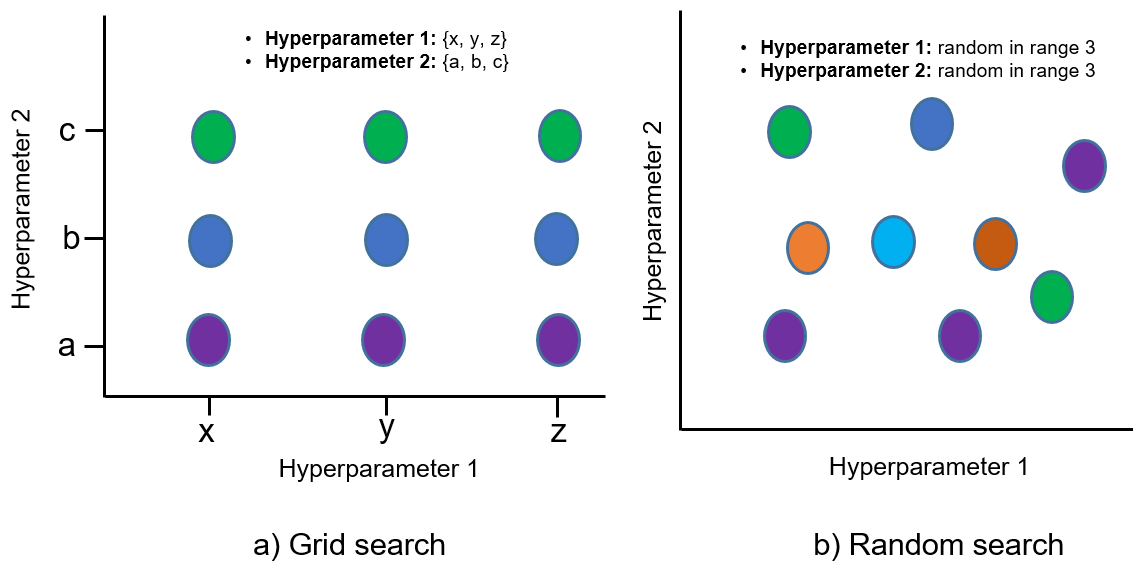
\includegraphics[width=0.8\textwidth]{images/gvr.png}\\ 
    \scriptsize{
        \textbf{Random search:} $x$-squared number of values are picked randomly and used in cross validation to test the accuracy of the experiment for each combination.
        } 
\end{tcolorbox}

\subsection{Techniques for hyperparameter optimization}
Since an appropriate selection of hyperparameters have huge impact on the performance of ML model, `hyperparameter tuning' is performed, which is the process of searching best model based on optimal combination of hyperparameters. In other words, hyperparameter optimization~(HPO) is the problem of choosing the best combination~(or optimal) hyperparameters for a learning algorithm. HPO is often represented as the following objective function: 

\vspace{-6mm}
\begin{align}
    x^{\star}=\arg \min _{x \in \mathcal{X}} f(x)
    \label{eq:hpt}
\end{align}

where $x \in X$, $f(x)$ represents an objective score to minimize, e.g. RMSE evaluated on the validation set and $x^*$ is the set of hyperparameters to yield the lowest value of the score. However, in case of complex model, there are more than one hyperparameter on which there are several approaches to perform hyperparameter tuning such as grid search, random search, and Bayesian optimization. \\

\subsection{Grid search and random search}
In grid search, evenly spaced values are generated for each hyperparameter being tested, followed by building a model for each possible combination of all of the hyperparameter values, evaluating each model and selecting the architecture which produces the best results. %\subsection{Random search}
In random search, random values for each hyperparameter are generated that are used in cross-validation to evaluate the model for each combination.

\hspace*{3.5mm} Random search is better than grid search for most cases, hyperparameters are not equally important, making some hyperparamters are more important than others. A Gaussian process analysis of the function from hyper-parameters to validation set performance reveals that for most data sets only a few of the hyper-parameters really matter, but that different hyper-parameters are important on different data sets. This phenomenon makes grid search a poor choice for configuring algorithms for new data sets. %- Bergstra, 2012

\subsection{Bayesian optimization} 
Both grid search and random search perform individual experiments while training the model with various hyperparameter values and observe in each case. Many optimization problems in ML are black box optimization problems, where the objective function $f(x)$ in \cref{eq:hpt} is a black box function~\cite{BO}, making it's difficult to know it's analytical expression for $f$ nor do we know its derivatives. Oftentimes, evaluation of the function is restricted to sampling at a data point $x$ and getting a possibly noisy response~\cite{BO}.
Nevertheless, as each experiment using grid search and random search is performed separately, reusing the result of current experiment to improve the next one is not possible. However, they can easily be parallelized by employing an approach called ``Bayesian optimization"~(BO), which belongs to a class of sequential model-based optimization algorithms. BO allows using the results of the previous iteration to improve the sampling method of the next experiment.

\hspace*{3.5mm} BO incorporates prior belief about $f(x)$ and updates the prior with samples drawn from $f(x)$ to get a posterior that better approximates $f(x)$. The model used for approximating the objective function is called surrogate model. In BO, a model is initially defined and trained with hyperparameters $\sigma$, which is scored $v$ w.r.t some evaluation metrics. The previously evaluated hyperparameter values are reused to compute a posterior expectation of the hyperparameter space. Optimal hyperparameter values are then chosen according to this posterior expectation as the next model candidate, which is repeated iteratively until converging to an optimum. Gaussian process is employed to model the prior probability of model scores across the hyperparameter space. 
%This model then enables to use the hyperparameter values $\sigma_1,\sigma_2,...,\sigma_n$ and corresponding scores $v_1,v_2,...,v_n$ to approximate a continuous score function over the hyperparameter space. %It includes the degree of certainty of the estimate, which can be used to identify the candidate hyperparameter values, which hopefully would yield the largest expected improvement over the current score. 
BO finds a better optimum in a smaller number of steps than random search and beats the baseline in almost every run~\cite{BO}. Nevertheless, this becomes even more evident in higher-dimensional search spaces, e.g., imagine that geneomics data often have 20K+ dimensionality. 

\section{Interpretability of ML Models}
Although DL models have shown tremendous success at AI-aided diagnosis and prognosis, showing high effectiveness and accuracy. However, there are many cases where not only high accuracy, but also explanation about the outcome is necessary. Suppose, we have an accurate model that can classify cancerous samples with an accuracy of 90\%. Still, we cannot claim that it has high confidence, given that the single accuracy metric is an incomplete description~\cite{doshi2017towards} and can't be enough in AI-aided diagnosis and prognosis, unless it explains the reason behind the  decision. Otherwise, such a model has to perceive a `black box' method as it cannot explain why it reached to such a diagnosis decision and lack of transparency.  

\hspace*{3.5mm} If the parameters $\boldsymbol{\theta}$ of a ML model $\boldsymbol{f}$ and it's architecture are known, the model is considered a `white-box'. %A white-box model also helps improve model-debugging and promotes trust. 
However, a `white-box' model is not necessarily explainable or interpretable~\cite{das2020opportunities}. On the other hand, an ML model $\boldsymbol{f}$ is considered a `black-box' if the model parameters and network architectures are hidden from the end-user. Based on this intuition, we can slightly coined the definitions of `black-box' and `white-box' provided by Das et al.~\cite{das2020opportunities} models as follows: 

\begin{definition}
    \textbf{white-box model}: a ML model $f$ is `white-box': i) if its parameters $\boldsymbol{\theta}$ and architecture are known to the end users, and ii) users have sufficient know-how and why it provides decision/prediction.  
\end{definition}

\begin{definition}
    \textbf{black-box model}: a ML model $f$ is considered black-box' if the model parameters and network architectures are hidden from the end-users. 
\end{definition}

\hspace*{3.5mm} In contrast, interpretable ML refers to methods that make the behavior and predictions of a system understandable to humans~\cite{molnar2019interpretable}. 
%This is a serious drawback since interpretability is essential to generate insights on why a given cancer case is of a certain type, and since knowing the most important biomarkers can help in recommending more accurate treatments and drug repositioning. 
%Further, the `right to explanation' of the EU GDPR~\cite{kaminski2019right} gives patients the right to know why and how an algorithm made a diagnosis decision. However, existing approaches can neither ensure the diagnosis transparently nor are they trustworthy. 
%AI-aided system has to be well-interpretable and explainable.
Interpretability of an ML system is the ability to explain or to present in understandable terms to a human~\cite{doshi2017towards}. Following is a non-technical definition by Miller et al.~\cite{XAI_miller}. Although a white-box model improves model-debugging and promotes trust, knowing it's architecture and parameters alone won't make the model essentially explainable~\cite{das2020opportunities}.  %~(\cref{def:xai_1}) and Kim et al.~\cite{XAI_kim}~(\cref{def:xai_2}), respectively:

\begin{definition}
    \textbf{interpretability}: is the degree to which a human can understand the cause of a decision.
    \label{def:xai_1}
\end{definition}

\iffalse
\vspace{-6mm}
\begin{definition}
    \textbf{interpretability}: is the degree to which a human can consistently predict model's result.
    \label{def:xai_2}
\end{definition}
\fi 
\vspace{-6mm}
\hspace*{3.5mm} Model interpretation is an extension of the model evaluation, which helps to foster a better understanding of a model’s learned decision policies and gives the ability to explain a model in a way which is human understandable such that the outcomes are self-descriptive and needs no further explanation. 
The higher the interpretability, the easier it is for someone to comprehend why a particular decision or prediction is made by the model~\cite{stiglic2020interpretability,bhatt2020explainable}, i.e., trustworthiness for the human. In either way, good interpretability has to be ensured both locally, e.g., individual predictions and globally, e.g., entire model behavior. 

\begin{figure*}[h]
	\centering
	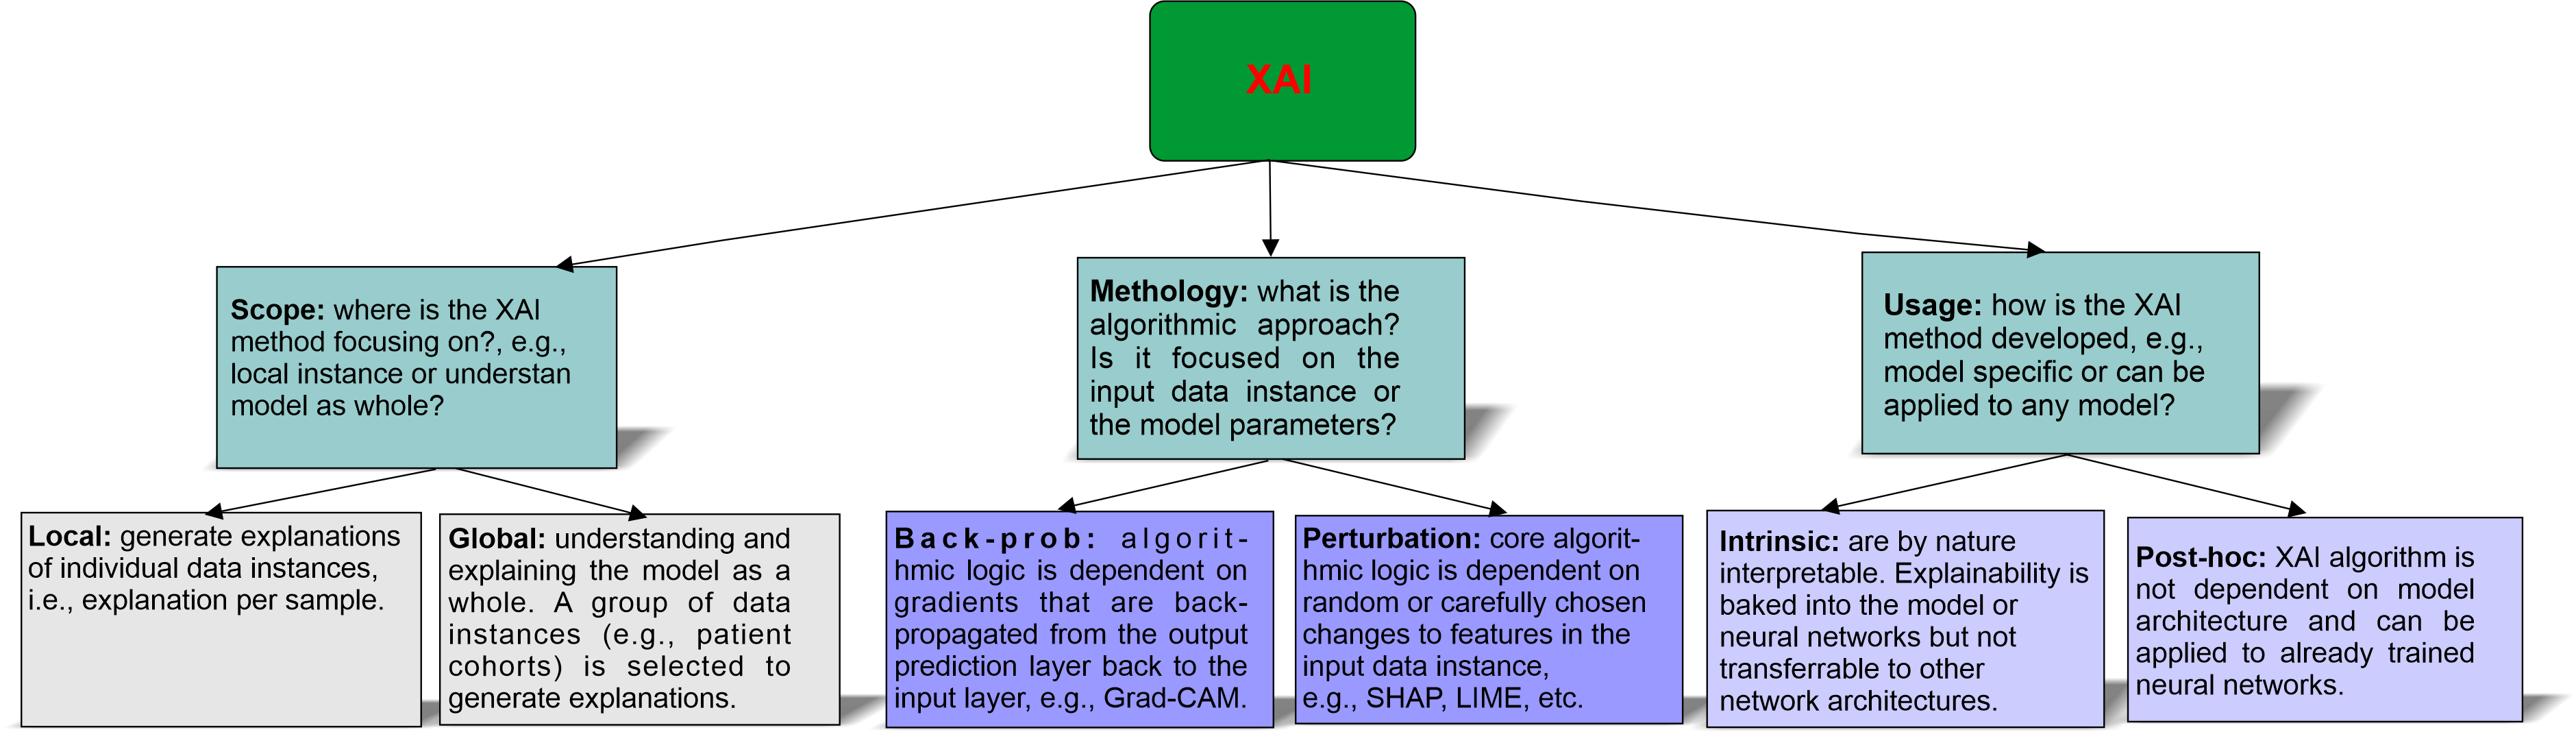
\includegraphics[width=\textwidth,height=70mm]{images/xai_tec.png}	
    \caption{Categorization of the survey in terms of scope, methodology, and usage~(based on~\cite{das2020opportunities})}	
	\label{fig:survey_xai}
\end{figure*}

\hspace*{3.5mm} Although many authors used interpretability and explainability interchangeably, the former means that the cause and effect~(e.g., of a certain outcome) can be determined in a system. The latter is the extent to which the internal working mechanism of an AI system can be explained to humans, in human-interpretable language. Miller et al.~\cite{miller2018explanation} defined explanation as the answer to a why and how questions. For example, in our cancer diagnosis context, a patient may have the following questions: i) why do I have colon cancer?, ii) Why did not the treatment work on me?, iii) how did the model predict that I have colon cancer?, etc. However, there is a trade-off between explianability and accuracy. How well does an explanation predict unseen data is a measurement of accuracy~\cite{molnar2019interpretable}. High accuracy is important if the explanation is used for predictions in place of the ML model. However, if the goal is to explain what the `black-box' model does~(i.e., algorithmic transparency), only `fidelity' is important~\cite{molnar2019interpretable}. 

\subsection{Algorithmic transparency}
A ML model is considered transparent if it is expressive enough to be human understandable, where transparency can be a part of the algorithm itself or using external means~(e.g., model
decomposition or simulations)~\cite{das2020opportunities}. 
Although the phrase `algorithmic transparency' was coined by Nicholas Diakopoulos et al.~\cite{diakopoulos2017algorithmic} in 2016 w.r.t role of algorithms in deciding the content of digital journalism, the underlying principle dates back to 1970s and the rise of automated systems for scoring consumer credit~\cite{diakopoulos2015algorithmic}.  %\footnote{\url{https://en.wikipedia.org/wiki/Algorithmic_transparency}}. 

\begin{definition}
    {\textbf{algorithmic transparency}} is the principle that the factors that influence the decisions made by algorithms should be visible, or transparent, to the people who use, regulate, and are affected by systems that employ those algorithms.
\end{definition}

\hspace*{3.5mm} More technically, ``algorithmic transparency" is how the algorithm learns a model from the data and maps different relationships transparently based on what it makes prediction for unknown samples. First example could be a decision tree algorithm, which implicitly performs variable screening or feature selection. Hence, feature importance is clear, showing clear interactions between features. The second example could be image classification using neural networks, e.g., while classifying images, a CNN model learns features~(e.g., class-discriminating pixels) using edge detectors and filters across convolutional layers. Then it can learn more abstract features in the deepest layer. Then it can provide attention on some areas using attention maps, explaining where most important pixels are located to. \\

\vspace{-2mm}
\begin{tcolorbox}[colback=white!3!white,colframe=gray!120!black,title=\faBook~Algorithmic transparency]
    %INFO: \faBook \\
    \scriptsize{
        \textbf{Algorithmic transparency:} is how a learning algorithm learns a model from the data by mapping relations to make prediction for unknown sample.
        }
\end{tcolorbox}

\hspace*{3.5mm} These are a few ways to transparently show how the algorithm works. Some models are inherently interpretable, some are not. For example, DNNs that are propagating gradients through a network with millions of weights are less understood because of their inner workings, are less transparent~\cite{molnar2019interpretable}. However, they way a linear~(linear or logistic regression) or tree-based model~(decision trees) learn is very transparent and is characterized by a high transparency. Algorithmic transparency requires only knowledge of the algorithm, not of the data or learned model itself~\cite{molnar2019interpretable}. Implicitly, ``algorithmic transparency" also means that the inputs used by the algorithm must be known, but they necessarily need not be fair. 

\subsection{Needs for interpretability}
Although, not every predictions made by a ML algorithm needs to be explained, explainable ML is essential for future customers, trust, and effectively manage the emerging generation of AI applications~\cite{das2020opportunities}. In general, ML models needs to be interpretable, higher interpretability of the model means easier comprehension and explanation of future predictions for end-users~\cite{stiglic2020interpretability}. With the wider usage of AI in numerous domains, the need to explain an ML model result is important for ethical, judicial, as well as safety reasons~\cite{das2020opportunities}. Literature have discussed important aspects showing the importance of the XAI. Among others, three most important concerns identified by Das et al.~\cite{das2020opportunities} are trustability, transparency, and 3) fairness of AI algorithms. \Cref{fig:need_for_xai} depicts some requirements for explainability and transparency. 
%Current business models include interpretation as a step before serving the ML models on production systems, however are often limited to small tree-based models. With the use of highly nonlinear deep learning algorithms with millions of parameters in ML pipelines, XAI techniques must improve all three concerns mentioned above. 
%However, interpretability stems from an incompleteness in the problem formalization, which evolves a fundamental barrier to optimization and evaluation~\cite{doshi2017towards}. Note that incompleteness is distinct from uncertainty: the fused estimate of a missile location may be uncertain, but such uncertainty can be rigorously quantified and  formally reasoned about. In ML terms, we distinguish between cases where unknowns result in quantified variance—e.g. trying to learn from small data set or with limited sensors—and incompleteness that produces some kind of unquantified bias—e.g. the effect of including domain knowledge in a model selection process. In short, interpretability is desired and essentials in several aspects, e.g., scientific understanding and ethics.

\iffalse
\begin{figure*}[h]
	\centering
	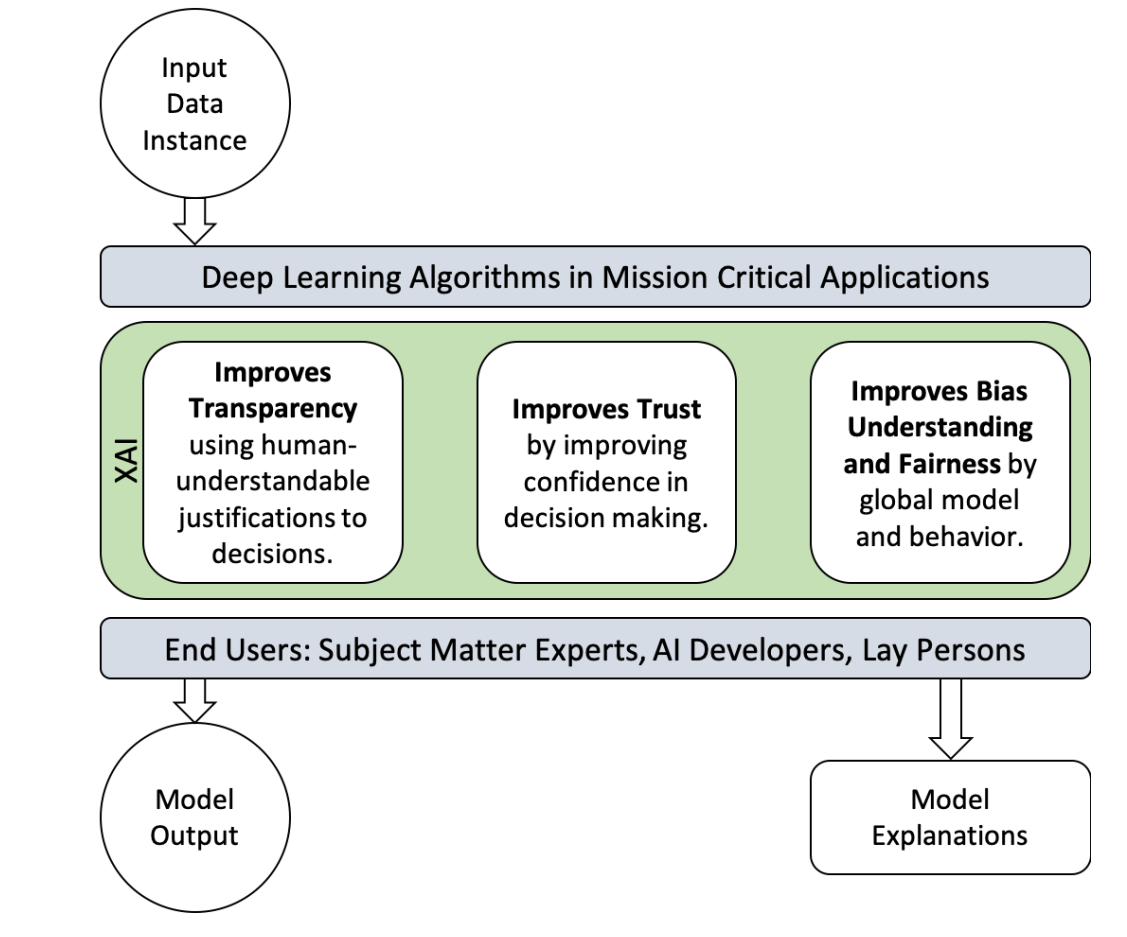
\includegraphics[width=\textwidth,height=40mm]{images/adv_xai.png}	
    \caption{Significant expected improvements when using XAI techniques to support decision making of end-users. We believe XAI is important due to improvements in trust, transparency, and in understanding bias and fairness.~(based on~\cite{das2020opportunities})}	
	\label{fig:survey_xai}
\end{figure*}
\fi 

\begin{figure*}[h]
	\centering
	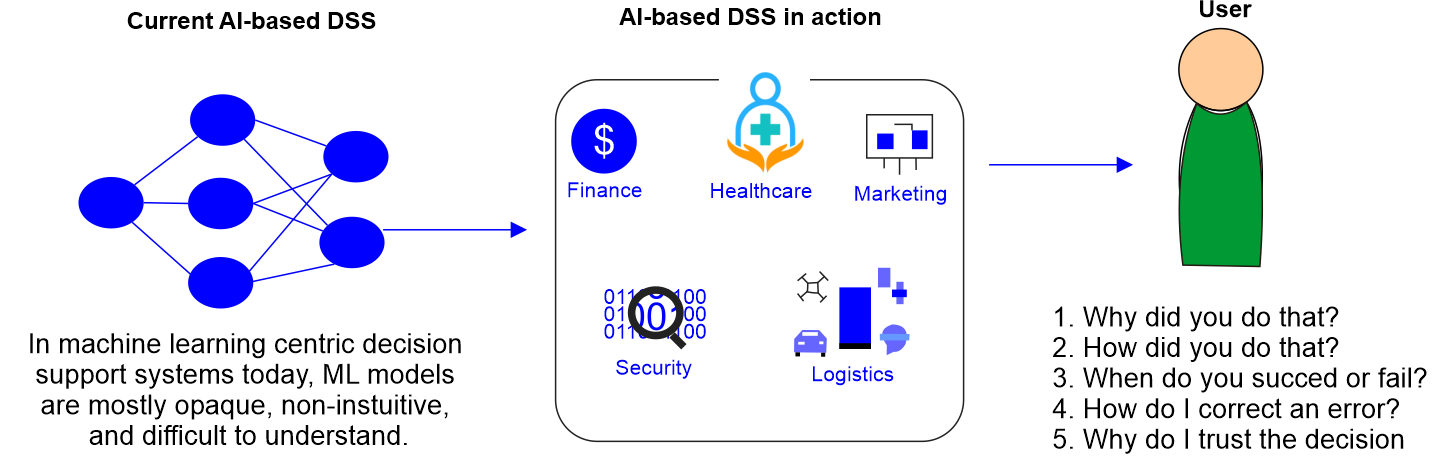
\includegraphics[width=\textwidth,height=55mm]{images/why_xai.png}	
    \caption{Needs for explainability and transparency in DSS}	
	\label{fig:need_for_xai}
\end{figure*}

\hspace*{3.5mm} XAI techniques improve transparency fairness by creating a human-understandable justification to the decisions and could find and deter adversarial examples if used properly~\cite{das2020opportunities}. XAI techniques can improve trust. Trustability of a ML model is a measure of confidence in the intended working of a given model in dynamic real-world environments. Often decisions and judgements are primarily based on the knowledge and available explanations to situations and the trust we generate. A scientific explanation or logical reasoning for a sub-optimal decision is better than a highly confident decision without any explanations~\cite{das2020opportunities}. XAI techniques improve fairness by mitigating different types of bias. While bias in ML realm indicate the disproportionate weight, prejudice, favor, or inclination of the learnt model towards subsets of data due to both inherent biases in human data collection and deficiencies in the learning algorithm, fairness is the quality of a learned model in providing impartial decisions without favoring any populations in the input data distribution~\cite{das2020opportunities}.
Eventually, XAI promotes fairness and helps mitigate biases introduced to the AI decision either from input datasets or poor neural network architecture.

\hspace*{3.5mm} Further, article 14 of EU GDPR states that when a company uses automated decision-making tools, it must provide ``meaningful information about the logic involved, as well as the significance and the envisaged consequences of such processing for the data subject.” In short, the GDPR prohibits the use of ML for automated decisions unless a clear explanation of the logic used to make each decision is well-explained. This is, however, not possible with conventional ML, mainly, due to the black-box nature. In case of employing ML for profiling and automated decisions, and are subject to the GDPR, five things have to be ensured~\cite{doshi2017towards}: i) to identify processes in your business that use profiling and automated decisions, ii) to inventory the ML models currently used, iii) to assess your existing models. Are they interpretable? Can you demonstrate to an auditor that they do not discriminate?, iv) to assess your current ML techniques. Do they produce interpretable rules?, and v) to develop a strategy for meeting compliance requirements in each stage of the ML workflow. \\

\subsection{Scopes and implementation levels for interpretability}
A wide range of strategies for interpretable ML have been developed and applied to problems in genetics and genomics, ranging from model-agnostic to model-specific. They often characterized based on if they provide global or local interpretations~\cite{azodi2020opening}. In other words, depending on the abstraction, two types of interpretability can be achieved: local interpretability and global interpretability. The former can explain a single prediction, while the latter is to explain entire model behaviour~\cite{molnar2019interpretable}. \Cref{fig:survey_xai} shows the categorization of the survey in terms of scope, methodology, and usage~(based on~\cite{das2020opportunities}). 
Local interpretability of an ML model can be achieved by designing justified model architectures that explains why a specific decision was made or by providing similar examples of instances to the target instance~\cite{stiglic2020interpretability}. For example, for our cancer diagnosis use case, by emphasizing specific characteristics of a patient that represents the characteristics of a smaller group of cancer patients such as breast cancer, yet different in other patients~(rather than all the patients in a dataset).

\vspace{1mm}
\begin{tcolorbox}[colback=white!3!white,colframe=gray!120!black,title=\faBook~Local vs. global interpretation]
    %INFO: \faBook \\
    \scriptsize{
        \textbf{Global interpretability:} how does the trained model make predictions~\cite{molnar2019interpretable}? \\
        \textbf{Global interpretation:} being able to explain the conditional interaction between dependent and independent variables based on the training set, i.e., it involves explaining the overall relationship between features and labels.
        } \\ \\
    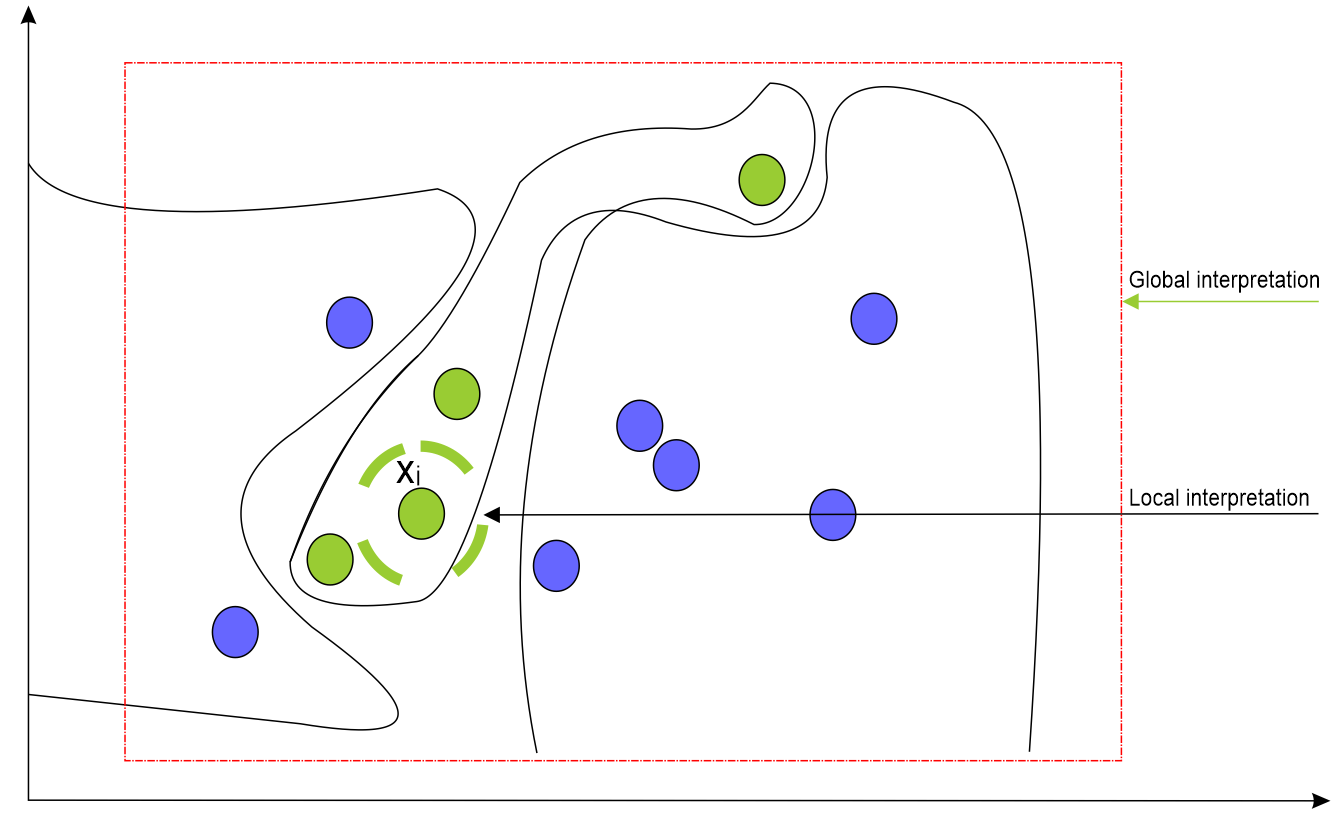
\includegraphics[width=0.6\textwidth,height=60mm]{images/lvg.png}\\ 
    \scriptsize{
        \textbf{Local interpretability:} why did the model make a certain prediction for an instance~\cite{molnar2019interpretable}? \\
         \textbf{Local interpretation:} being able to explain the conditional interaction between dependent and single prediction, i.e., focuses on explaining the prediction of an individual instance. 
        } 
\end{tcolorbox}

\hspace*{3.5mm} In contrast, global interpretability signifies the overall transparency of the model inside a model on an abstract level. Nevertheless, an interpretable ML can be developed that can have cohort-specific interpretability, where they focus on population subgroups~\cite{stiglic2020interpretability}. However, we can also classify such cases as either global if the subgroup is treated as the sub-population or as local if single prediction interpretations for the subgroup are grouped together~\cite{molnar2019interpretable}. 

\begin{figure*}[h]
	\centering
	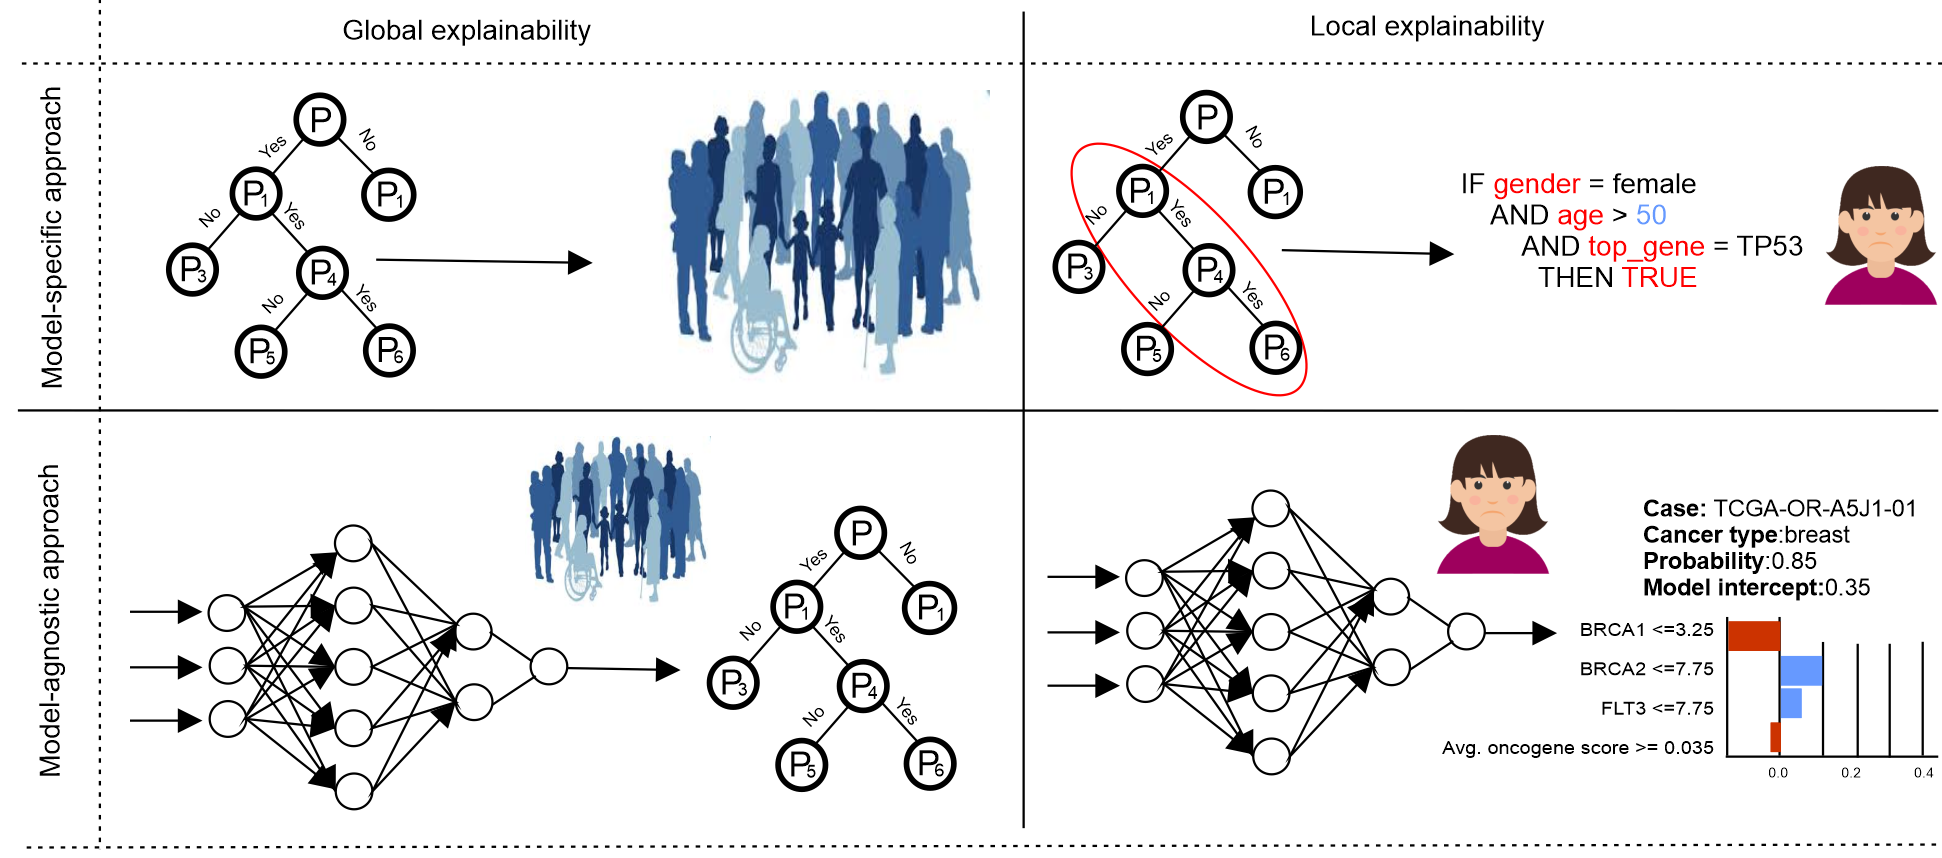
\includegraphics[width=0.9\textwidth,height=70mm]{images/lvg_cancer.png}	
    \caption{Scopes and types of ML models in healthcare based on their interpretability characteristics~(based on~\cite{stiglic2020interpretability}, showing an example of cancer types prediction}	
	\label{fig:local_vs_global_ex}
\end{figure*}

\hspace*{3.5mm} A more concrete example related to our cancer genomics would be as follows: suppose, we train an ML model to predict if a gene is up-regulated~(i.e., label) after some treatment based on the presence or absence of a set of regulatory sequences~(i.e., features). While a global interpretation strategy will tell you how important regulatory sequence $X_i$ is for predicting up-regulation across all genes in the dataset, whereas a local interpretation strategy will tell you how important regulatory sequence $X_i$ is for predicting gene $y_i$ as up-regulated. As Azodi et al~\cite{azodi2020opening} suggest, we should also emphasize that ML models identify association through correlation. This implicitly means that ML interpretation strategies do not necessarily meant to identify causal relationships between input features and labels. %\subsection{Model-specific vs. model-agnostic interpretability}
As illustrated in \cref{fig:local_vs_global_ex}, local and global interpretations can be derived in two separate ways: model-specific and model-agnostic. The former is limited to specific models by which the explanations can be derived by examining internal model parameters~\cite{stiglic2020interpretability}. The latter is, however, applicable on any ML model in a post-hoc manner~\cite{molnar2019interpretable}. 

\iffalse
\begin{figure*}[h]
	\centering
	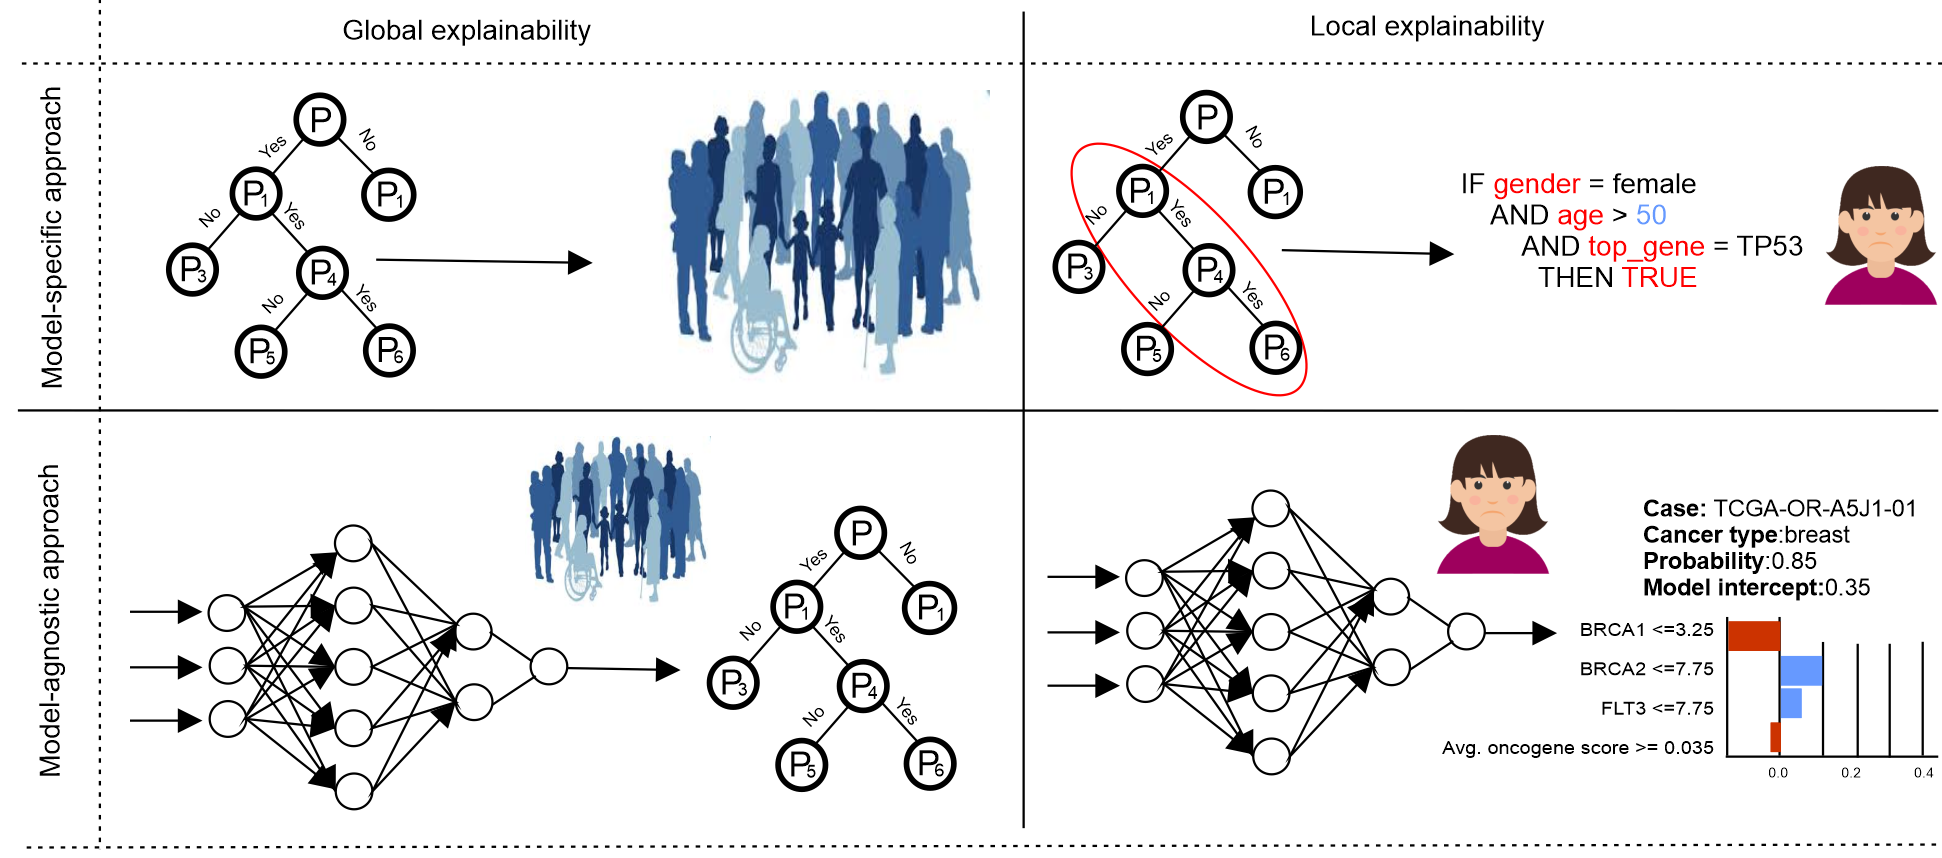
\includegraphics[width=\textwidth,height=70mm]{images/lvg_cancer.png}	
    \caption{Types of ML models in healthcare based on their interpretability characteristics (based on~\cite{stiglic2020interpretability}, showing an example of cancer types prediction}	
	\label{fig:local_vs_global_ex}
\end{figure*}
\fi 

\vspace{2mm}
\begin{tcolorbox}[colback=white!3!white,colframe=gray!120!black,title=\faBook~Model surrogate]
    %INFO: \faBook \\
    \scriptsize{
        \textbf{Surrogate strategies:} model surrogation is a model interpretation strategies, which involve training an inherently interpretable model using the same data as a `black-box' model to approximate the predictions of the `black-box' model. }
\end{tcolorbox}

\subsection{Techniques for interpretability}
Based on outputs returned by the black-box model, \textit{surrogate} or a simple proxy model is often developed to learn a locally faithful approximation of a complex model~\cite{stiglic2020interpretability}. Besides, probing and perturbing are also used as ML interpretation strategies. The way of interpreting a model's outcome can also be classified according to the results of the prediction model, e.g., following ways are outlined by Molnar et al.~\cite{molnar2019interpretable}:

\vspace{-2mm}
\begin{itemize}[noitemsep]
    \item \textbf{Feature summary statistics}: summary of each feature and their impact on the model predictions. 
    \item \textbf{Feature summary visualization}:  summary of the methods used to visualize and in order to make the visual communication easier, where outcomes are  presented with bars, plots, or table. 
    \item \textbf{Model internals approach}: the interpretation of intrinsically interpretable models, such as linear models in which model weights represent both internals parameters and summary statistics for the features. However, typically, internal parameters of model-agnostic models are not inspected~\cite{molnar2019interpretable}. 
    \item \textbf{The data point interpretability}: methods that require data points themselves to allow interpretability to  return data points to make model interpretable. 
\end{itemize}

\hspace*{3.5mm} To explain and interpret the model predictions these ways, several approaches and methods have been proposed. 
\Cref{fig:xai_timeline} shows a timeline of XAI algorithms, covering scopes, methodology, and usage level~(based on~\cite{das2020opportunities}). In this subsection, we'll briefly cover most widely used ones. 

\subsubsection{Feature-based attribution methods}
\label{subsubsec:FI_shap}
For the human-level interpretability of a model, we need to know the inner insights, e.g., what features does a model think are most important and significant? Some of the features have higher impact than the others. This concept is called feature importance, which can be computed based on permutation importance~(PI). Intuitively, we can think of such importance both locally and globally (see in local vs global interpretability), e.g., for a single prediction, we can compute the effect of each feature in the data, or, effect of each feature over a large number samples and overall the predictions.

\begin{sidewaysfigure*}
	\centering
	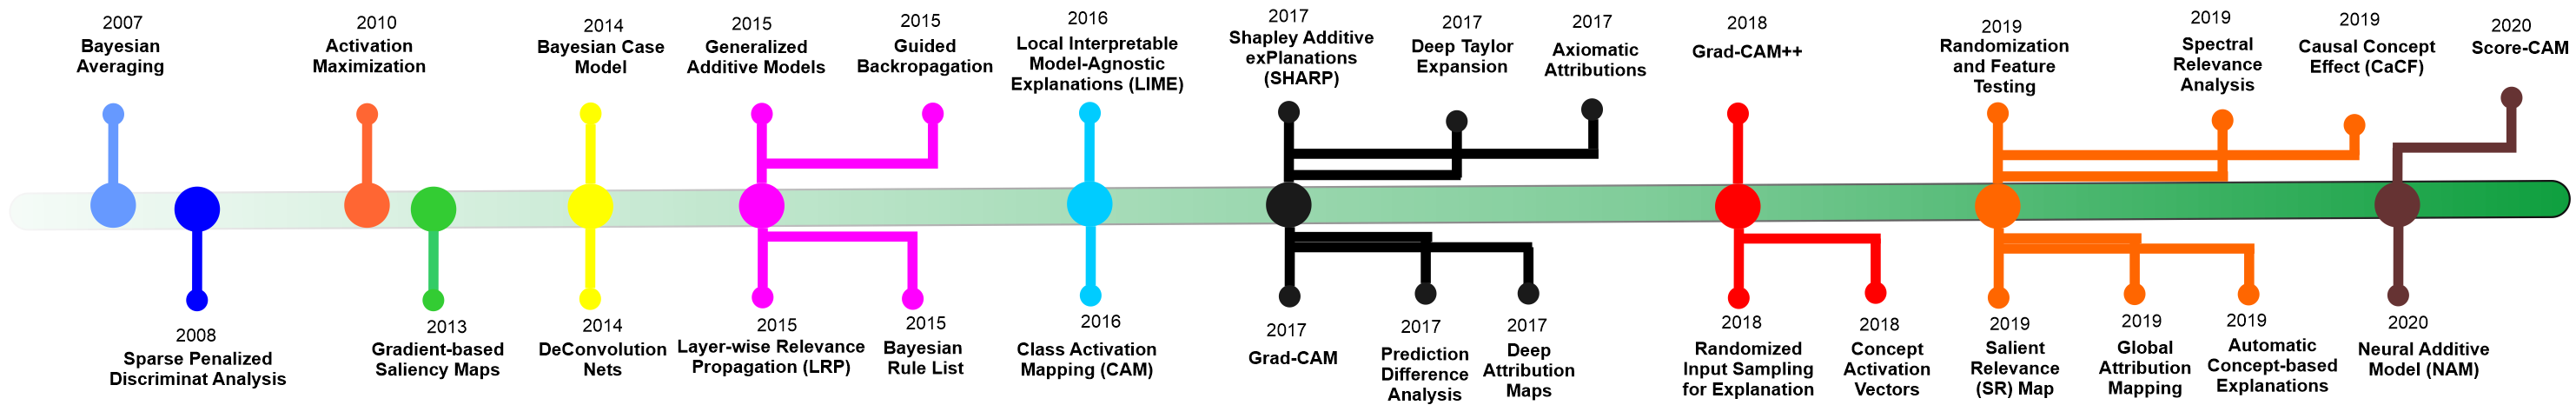
\includegraphics[width=0.9\textwidth,height=55mm]{images/xai_roadmap.png}	
    \caption{A timeline of XAI algorithms, covering scopes, methodology, and usage level~(based on~\cite{das2020opportunities})}	
	\label{fig:xai_timeline}
\end{sidewaysfigure*}

\hspace*{3.5mm} Feature importance methods define an explanation function $g: F \times \mathbb{R}^{d} \mapsto \mathbb{R}^{d}$ that takes in a model $F$ and a point of interest $x$ and returns importance scores $g(F,x) \in \mathbb{R}^{d}$ for all features is the importance or attribution for feature $x_i$ of sample $x$. In other words, PI works by randomly permuting or shuffling a single column in the validation dataset leaving all the other columns intact, where a feature is considered ``important” if and only if the model's accuracy drops significantly and the error is increased. On the other hand, a feature is considered ``unimportant’ if shuffling its values does not affect the model's accuracy significantly. Explanation functions roughly fall into two categories: i) perturbation-based techniques, ii) saliency map and gradient-based techniques. 

\hspace*{3.5mm} A widely used perturbation based methods is based on Shapley values inspired by cooperative game theory. A Shapley Value is the average marginal contribution of a feature value over all possible combinations of features which are used to estimate the Shapley value of a specific feature, whereas Shapley values are a way to distribute the gains to its players. SHapley Additive exPlanations (aka. SHAP) is a unified approach to explain the output of any ML model. SHAP connects game theory with local explanations, uniting several previous methods and representing the only possible consistent and locally accurate additive feature attribution method based on expectations~\cite{NIPS2017_7062}. 

\subsubsection{Saliency map and gradient-based attribution methods}
The saliency map and gradient-based attribution methods are used to identify relevant regions and assign importance to each input feature, e.g., pixel for image data. Typically first-order gradient information of a complex model w.r.t is used to produce maps that indicate the relative importance of the different input features for the classification. Gradient-weighted class activation mapping~(Grad-CAM)~\cite{selvaraju2017grad}, it's improved variant called Grad-CAM++~\cite{chattopadhay2018grad}, sensitivity analysis~(SA)~\cite{baehrens2010explain, simonyan2013deep}, and layer-wise relevance propagation (LRP) are examples of this category. 

\subsubsection{Sensitivity analysis}
SA explains a prediction based on the model's locally evaluated gradient, aka. partial derivatives~(PD). Mathematically, SA quantifies the importance of each input variable $i$~(at low level, e.g., image pixel) $R_{i}=\left\|\frac{\partial}{\partial x_{i}} f(\mathbf{x})\right\|$. This measure assumes that most relevant input features are those for which the output is sensitive. Usually, a heatmap~(HM) is plotted to visualize and indicate which pixels need to be changed to make the image look similar to the predicted class. However, such HM does not indicate which pixels are actually pivotal for a specific prediction. Consequently, SA is not suitable for quantitative evaluation. 

\subsubsection{Grad-CAM, Grad-CAM++, and Score-CAM}
Guided backpropagation~(GB)~\cite{springenberg2014striving} is another method, where absolute values of the gradient of the output with respect to the input nodes are shown as heatmap, with the additional twist that negative gradients are set to zero at the rectification layers of the network is based on the fact is ``rectifying” the gradients in the backward pass leads to more focused heatmap~\cite{bohle2019layer}. While class-discriminating attention map visualization are appended to exhibit significant features for class assignment. To overcome the opaqueness of CNN, class activation maps (CAM)~\cite{zhou2016learning} is proposed. 

\hspace*{3.5mm} To explain where the model provides more attention, CAM computes the amount of weights of each feature map from the final conv layer. CAM calculates the contribution to prediction $y_c$ at location $(i,j)$, where the goal is to obtain $L_{ij}^{c}$ that satisfies $y^{c}=\sum_{i, j} L_{ij}^{c}$. The last feature map $A_{ijk}$ and prediction $y_c$ are represented in a linear relationship in which linear layers consist  of global average pooling (GAP) and FCL: i) GAP outputs $F_{k}=\sum_{i,j} A_{ijk}$, ii) FCL that holds weight $w_{k}^{c}$, generates the following output~\cite{kim2020extending}: 
 
 \vspace{-2mm}
 \begin{align}
     y^{c}=\sum_{k} w_{k}^{c} F_{k}=\sum_{k} w_{k}^{c} \sum_{i, j} A_{i j k}=\sum_{i, j} \sum_{k} w_{k}^{c} A_{i j k}.
 \end{align}
 \vspace{-2mm}
 
\noindent where $L_{i j}^{c}=\sum_{k} w_{k}^{c} A_{i j k}$~\cite{kim2020extending}. Subsequently, heat maps~(HM) are then plotted to visualize the weighted combination of the feature maps. However, if linear layers replace the classifier architecture, re-training of the network is required and non-linearity of classifier vanishes. Subsequently, literature~\cite{114} came up with an efficient generalization of CAM called Grad-CAM, where instead of pooling, globally averages gradients of feature maps as weights, w.r.t, aiming at class $c$. The guided backpropagation in Grad-CAM helps to generate more human-interpretable but fewer class-sensitive visualizations than the saliency maps~(SM)~\cite{nie2018theoretical}. Since SM use true gradients, trained weights are likely to impose a stronger bias towards specific subsets of the input pixels. Accordingly, class-relevant pixels are highlighted rather than producing random noise~\cite{nie2018theoretical}. Therefore, Grad-CAM is used to draw the HM to provide attention to discriminating regions, where the class-specific weights of each FM are collected from the final conv layer through globally averaged gradients~(GAG) of FMs instead of pooling~\cite{chattopadhay2018grad}: 

\vspace{-2mm}
\begin{equation}
    \alpha_k^c=\frac{1}{Z}\sum_{i}\sum_{j}\frac{\partial y^c}{\partial A_{ij}^k}.
    \label{eq:alpha}
\end{equation}
\vspace{-2mm}

where $Z$ is number of pixels in a FM, $c$ is gradient of the class, and $A_{ij}^k$ is the value of $k^{th}$ FM. Having gathered relative weights, the coarse SM, $L^c$ is computed as the weighted sum of $\alpha_k^c*A_{ij}^k$ of the ReLU activation and employ the linear combination to the FM, as features with only positive influence on the class are of interest~\cite{chattopadhay2018grad} and negative pixels that belong to other categories in the image are discarded~\cite{114}:

\vspace{-2mm}
\begin{equation}
    L^c=\operatorname{ReLU}(\sum_{i}\alpha_k^cA^k).
    \label{3.11}
\end{equation}
\vspace{-2mm}

\hspace*{3.5mm} However, if an image contains multiple occurrences with slightly different orientations or views of the same class, several objects would fade away in the saliency map created by Grad-CAM. Moreover, due to its overlooking at significance disparity among pixels, parts of objects are rarely focused by Grad-CAM. Grad-CAM++ is proposed~\cite{chattopadhay2018grad} to replace the GAG with a weighted average of the pixel-wise gradients since the weights of pixels contribute to the final prediction by applying the following iterators over the same activation map $A^k$, $(i,j)$ and $(a,b)$:

\vspace{-2mm}
\begin{align}
    \begin{aligned}
        w_{k}^{c}=\sum_{i} \sum_{j} \alpha_{i j}^{k c} \cdot \operatorname{ReLU}\left(\frac{\partial y^{c}}{\partial A_{i j}^{k}}\right) \\
        y^{c}=\sum_{k} w_{k}^{c} \cdot \sum_{i} \sum_{j} A_{i j}^{k} \\
        \alpha_{i j}^{k c}=\frac{\frac{\partial^{2} y^{\ell}}{\left(\partial A_{i j}^{k}\right)^{2}}}{2 \frac{\partial^{2} y^{c}}{\left(\partial A_{i j}^{k}\right)^{2}}+\sum_{a} \sum_{b} A_{a b}^{k} \frac{\partial^{3} y^{c}}{\left\{\left(\partial A_{i j}^{k}\right)^{3}\right\}}}.
    \end{aligned}
\end{align}

\hspace*{3.5mm} Although, CAM variants managed to steer clear of back-propagating gradients all the way up to inputs, gradients are essentially propagated only till the final conv layer. Besides, Grad-CAM and Grad-CAM++ are limited to specific architectures that uses average-pooling layer to connect conv layers to FCLs. 
Gradient for a DNN architecture can not only be noisy but also tends to vanish due to saturation in Sigmoid or the flat zero-gradient region in ReLU. One of the consequences is that gradient of the output w.r.t input or internal layer activation may be noisy visually which causes problems in the plain SM~\cite{wang2020score}. 
\hspace*{3.5mm} These apply to both Grad-CAM and Grad-CAM++. A recent approach called Score-CAM is proposed by Haofan Wang et al.~\cite{wang2020score}. While Grad-CAM and Grad-CAM++ use the gradient information flowing into the last convolutional layer to represent the importance of each activation map, Score-CAM utilizes the importance called Channel-wise Increase of Confidence~(CIC): Score-CAM considers a convolutional layer $l$ in a model $f$, given a class of interest $c$, \cref{3.11} can be rewritten $L_{\text {Score-CAM}}^{c}$ as follows: 

\begin{align}
    L_{S c o r e-C A M}^{c}=\operatorname{ReLU}\left(\sum_{k} \alpha_{k}^{c} A_{l}^{k}\right).
\end{align}

\hspace*{3.5mm} where $\alpha_{k}^{c}=C\left(A_{l}^{k}\right)$ and  $C(\cdot)$ denotes the CIC score for activation map $A_{l}^{k}$. Since the weights come from the CIC score corresponding to activation maps on target class, Score-CAM gets rid of the dependence on gradient. Score-CAM can localize both single and multi objects accurately. From application perspective, Grad-CAM tends to only capture one object in the image, Grad-CAM++ and Score-CAM can localize multiple objects, but SM of Score-CAM are more focused than Grad-CAM++~\cite{wang2020score}.

\subsubsection{Layer-wise relevance propagation}
LRP~\cite{LRP1} is based on an assumption that the likelihood of a class can be traced backwards through a network to the individual layer-wise nodes of the input~\cite{LRP2}. LRP identifies important pixels by running a backward pass in the neural network. The backward pass is a conservative relevance redistribution procedure, where nodes that contribute the most to the higher-layer receive most relevance from it. First, an image $x$ is classified in a forward pass. Relevance $R_{t}^{(L)}$ is then back-propagated using deep Taylor decomposition (DTD)~\cite{DTD} to generate a relevance map $R_{LRP}$. Assuming the network has $L$ layers and for layer $l$, $1,2,...,N$ are the nodes, $1,2,..,M$ are the nodes in layer $l+ 1$. The relevance $R_{n}^{(l)}$ at node $n$ in layer $l$ is recursively defined as follows~\cite{LRP2}.  

\vspace{-2mm}
\begin{align}
    R_{n}^{(l)}=\sum_{m} \frac{a_{n}^{(l)} w_{n, m}^{+(l)}}{\sum_{n^{\prime}} a_{n^{\prime}}^{(l)} w_{n^{\prime}, m}^{+(l)}} R_{m}^{(l+1)}.
    \label{eq:rn}
\end{align}

However, node-level relevance in case of negative values is calculated using ReLU as follows~\cite{LRP2}:

\vspace{-2mm}
\begin{align}
    R_{n}^{(l)}=\sum_{m} \frac{x_{n}^{(l)} w_{n, m}^{(l)}-b_{n}^{(l)} w_{n, m}^{+(l)}-h_{n}^{(l)} w_{n, m}^{-(l)}}{\sum_{n^{\prime}} x_{n^{\prime}}^{(l)} w_{n^{\prime}, m}^{(l)}-b_{n^{\prime}}^{(l)} w_{n^{\prime}, m}^{+(l)}-h_{n^{\prime}}^{(l)} w_{n^{\prime}, m}^{-(l+1)}}.
    \label{eq:rn_neg}
\end{align}

The output layer relevance is calculated before the back-propagation as follows~\cite{LRP2}:

\vspace{-2mm}
\begin{align}
    R_{n}^{(L)}=\left\{\begin{array}{ll}
    {z_{t}^{(L)}} & {n=t}, \\
    {0} & {\text { otherwise.}}
    \end{array}\right.
    \label{eq:rn}
\end{align}

\hspace*{3.5mm} However, the shortcomings of LRP lies since it is only considered the target class for the calculation, which can lead to the miss-attribution of input regions to the relevance. To tackle the issue of discriminating the target object’s class with the non-target classes, a class contrastive improvement on LRP called contrastive LRP (CLRP) is proposed~\cite{LRP3}. However, by equally penalizing non-target classes, the relevance produced in CLRP is reduced to zero, which is due to equal weighting of the non-target nodes~\cite{ LRP2}. Conversely, SGLRP is designed to take advantage of the post-softmax probabilities, where the gradient of the softmax output $\hat{y}_{t}$ is computed w.r.t, intermediate value of each output node $z_{n}$ as the relevance of the output layer $R_{n}^{(L)}$. The corresponding relevance map $R_{SGLRP}$ is then defined similar to \cref{eq:rn},

\iffalse
\vspace{-2mm}
\begin{align}
    R_{n}^{(L)}=\left\{\begin{array}{ll}
    {z_{t}^{(L)}} & {n=t} \\
    {0} & {\text { otherwise }}
    \end{array}\right.
\end{align}
\fi 

where $R_{1}^{(1)}, \ldots, R_{n}^{(1)}, \ldots, R_{N}^{(1)}$ are the relevance values at the input layer calculated by \cref{eq:rn} and \cref{eq:rn_neg}, except for the output layer relevance $R_{n}^{(L)}$, which is calculated as the gradient of softmax~\cite{LRP2}:

\vspace{-2mm}
\begin{align}
        R_{n}^{(L)}=\frac{\partial \hat{y}_{t}}{\partial z_{n}}=\left\{\begin{array}{ll}
        {\hat{y}_{t}\left(1-\hat{y}_{t}\right)} & {n=t}, \\
        {-\hat{y}_{t} \hat{y}_{n}} & {\text { otherwise.}}
    \end{array}\right.
\end{align}

\subsubsection{Decision rules-based explanations}
Due to the nested non-linear and complex structure, DNN architectures are mostly opaque and perceived as `black box' methods. They not only suffer from lack of transparency but also cannot reason about their underlying decisions. A DNN produces a prediction, which is an outcome of a bunch of mathematical expressions chained together that represent the way inner layers of an algorithm. However, using a set of rule, it possible to explain a decision directly to human with the ability to look up the reason for a decision. \\

\vspace{-2mm}
\begin{tcolorbox}[colback=white!3!white,colframe=gray!120!black,title=\faBook~Decision rules]
    %INFO: \faBook \\
    \scriptsize{
    \textbf{Structure:} decision rules follow a general structure: IF conditions are met THEN make a certain prediction. \\
    \textbf{Number of condition:} a decision rule has at least one feature=value statement in the condition, with no upper limit and more statements can be added with an ‘AND’ operator. \\
    \textbf{Single or multiple decision rules:} although a combination of several rules can be used to make predictions, sometimes a single decision rule is enough to explain the whole outcome.
}
\end{tcolorbox}

\hspace*{3.5mm} A decision rule is a simple IF-THEN statement consisting of a condition called antecedent and a prediction~\cite{molnar2019interpretable}. If derived from intelligible features and the length of the condition is short, decision rules are probably the most interpretable prediction models. In particular, the IF-THEN structure semantically resembles natural language and the way how human think~\cite{molnar2019interpretable}. 

\hspace*{3.5mm} Consequently, interpreting the predicted body mass index~(BMI) with decision rules maybe very easy, can be explained in layman term, e.g., suppose that we have a simple model for predicting the BMI. This simple concept may not be well understood by patients~\cite{post2015patient}, whereas a simple decision rule can be effective, e.g., IF BMI $\geq$ 30~(condition), THEN you're obese~(prediction). Further explanations can be provided saying that ``an increased BMI is associated with risk for developing type 2 diabetes, hypertension, and cardiovascular disease". To summarize, once we have a transparent and easily explainable AI model, decision rules can be generated using a series of IF-THEN statements. In this thesis, one of the goals is to generate human-interpretable decision rules automatically based on self-explanatory logic for all decisions. 


\subsubsection{Neuro-symbolic reasoning and challenges of current XAI methods}
Alejandro B. A, et al.~\cite{arrieta2020explainable} outline the trade-off between interpretability and accuracy, i.e., between the simplicity of the information given by the system on its internal functioning, and the exhaustiveness of this description
cognitive sciences to create objectively convincing explanations.
Explanations are better when constrictive, i.e., a good explanation is not only indicates why the model made a decision $\mathrm{X}$, but also why it made decision $\mathrm{X}$ rather than decision $\mathrm{Y}$. 

\hspace*{3.5mm}It is also explained that probabilities are not as important as causal links in order to provide a satisfying explanation. Considering that `black-box' models tend to process data in a quantitative manner, it would be necessary to translate the probabilistic results into qualitative notions containing causal links. Besides, counterfactual explanations can help the user to understand the decision of a model. In such a scenario, combining connectionist and symbolic paradigms is a promising way to address this challenge. On one hand, connectionist methods are more precise but opaque. On the other hand, symbolic methods are popularly considered less efficient, albeit they offer following features:

\begin{itemize}[noitemsep]
    \item It is possible to establish reasoning rules to allow symbolic methods to be constrictive.
    \item The use of a $\mathrm{KB}$ formalized by an ontology allows data processing in a qualitative way.
    \item Being selective is less straightforward for connectionist models than for symbolic ones.
\end{itemize}

\hspace*{3.5mm}The representation of the external reality using symbols, it seems obvious that the use of the symbolic learning paradigm is appropriate to produce an explanation. Therefore, neuro-symbolic interpretability could provide convincing explanations while keeping or improving generic performance. %An efficient explainable model enables users see the explanations that were already deduced based on the background knowledge. 
Having a semantic representation of the knowledge can help a model to have the ability to produce explanations. 

\iffalse
\subsection{Library and frameworks for interpretability}
\subsubsection{LIME}
Local Interpretable Model-agnostic Explanations~(aka. LIME) is an interpretable library to explain the predictions of any classifier or regressor. LIME explains the predictions by approximating it locally with an interpretable model. Additionally, LIME is is capable of explaining black-box classifiers, with two or more classes. 
\subsubsection{SHAP} 

\subsection{Measurements for explainability}
Unfortunately, there is little consensus on what interpretability in ML is and how to evaluate it for benchmarking. Current interpretability evaluation typically falls into two categories: 

\begin{itemize}[noitemsep]
    \item The first evaluates interpretability in the context of an application: if the system is useful in either a practical application or a simplified version of it, then it must be somehow interpretable~\cite{bhatt2020explainable}. 
    \item The second evaluates interpretability via a quantifiable proxy: a researcher might first claim that some model class—e.g. sparse linear models, rule lists, gradient boosted  trees—are interpretable and then present algorithms to optimize within that class~\cite{miller2018explanation}. 
\end{itemize}

\hspace*{3.5mm} To large extent, both evaluation approaches rely on some notion of ``you’ll know it when you see it'' or ``seeing is believing''. The notions of interpretability meet the first test of having face-validity on the correct test set of subjects: human beings. However, this is too naive that leaves many kinds of questions unanswerable, e.g., ``are all models in all defined-to-be-interpretable"? and ``are all model classes equally interpretable"? The simplistic answer to these questions would be defining some metrics for evaluating such an XAI model. Robert Hoffman et al.~\cite{hoffman2018metrics} proposed the following metrics/methods for evaluating such an XAI model, which we will try to answer in \cref{chapter:fairness}:

\begin{itemize}[noitemsep]
    \item The goodness of the explanations
    \item Whether users are satisfied by explanations
    \item How well users understand the AI systems
    \item How curiosity motivates the search for explanations
    \item Whether the user's trust on the AI is appropriate
    \item How the human-XAI work system performs.
\end{itemize}
\fi 

\section{Cancer Growth and Metastasis}
\label{cancer_growth}
In order to develop a DSS for clinical or medical setting, we need to know the data as well as the mechanism for which the diagnosis decision will be made. 
In this section, we focus on the different types and subtypes of cancer and their growth and metastasis. The idea is to acquire some biological interpretations of the genomics data. First of all, cancer is an umbrella term for a large group of diseases caused when abnormal cells divide rapidly, and spread to other tissue and organs. Consequently, changes such as mutations happened to the DNA in the cells, but usually cells correct these mistakes. When a mistake is not corrected, a cell can become cancerous. Mutations can cause cells that should be replaced to survive instead of die, and new cells to form when they're not needed. These extra cells can divide uncontrollably, causing growths called tumors to form. 

\hspace*{3.5mm} Besides, genetic mutations can be inherited. Cancer disrupts grow and divide process of healthy cells, which leads to abnormal growths~\cite{pancan}. 
%It’s caused by changes or mutations in DNA. DNA exists in the individual genes of every cell. It has instructions that tell the cell what functions to perform and how to grow and divide. 
Tumors can cause a variety of health problems, depending on where they grow in the body. Nevertheless, oftentimes cancer is caused by gene alterations and abnormal behaviors of genes that control cell division and cell growth. The change in the structure of occurring genetic aberrations, such as somatic mutations, CNV, profiles, and different epigenetic alterations are unique for each type of cancer~\cite{82Tomczak,19Cruz}. 
However, not all tumors are cancerous. Benign tumors are noncancerous and do not spread to nearby tissues. Sometimes, they can grow large and cause problems when they press against neighboring organs and tissue. Malignant tumors are cancerous and can invade other parts of the body. Some cancer cells can also migrate through the bloodstream or lymphatic system to distant areas of the body. This process is called metastasis.Cancers that have metastasized are considered more fatal and advanced than those that have not, hence are harder to treat. 

\hspace*{3.5mm} Cancers are named for the area in which they begin and the type of cell they are made of; even if they spread to other parts of the body, e.g., a cancer that begins in the lungs and spreads to the liver is still called lung cancer. On the other hand, cancer subtypes describes the smaller groups that a type of cancer can be divided into, based on certain characteristics of the cancer cells. Besides, there are several clinical terms used to describe certain types of cancer\footnote{\url{https://www.healthline.com/health/cancer\#types}}:

\begin{itemize}[noitemsep]
    \item \textbf{Carcinoma} is a cancer that starts in the skin or the tissues that line other organs.
    \item \textbf{Sarcoma} is a cancer of connective tissues, e.g., bones, muscles, and blood vessels.
    \item \textbf{Leukemia} is a cancer of bone marrow, which creates blood cells.
    \item \textbf{Lymphoma} and myeloma are cancers of the immune system.
\end{itemize} 

\hspace*{3.5mm} Although cancer is a lethal disease condition and more than 200 types of cancer have been identified, each of which can be characterized by different molecular profiles requiring unique therapeutic strategies~\cite{82Tomczak}. The most common types of cancer include, the cancer of bladder, breast, colon and rectal, endometrial, kidney, leukemia, liver, lung, melanoma, pancreatic, prostate, and thyroid. 

\section{Genomics Data-based Diagnosis of Cancer}
With high-throughput technologies such as next-generation sequencing~(NGS), cancer-
specific genetic profiling is now possible. The entire genome sequencing data using NGS can be used to identify similar genetic mutations and genetic variations associated with different tumors. %\subsection{Data availability}
As mentioned, different types of genomics data are used in cancer research, including somatic mutations, CNV, DNA methylation~(DM), gene expression~(GE), miRNA expression~(MR), and Isoform expression~(IEx), along with clinical outcomes. The largest uniformly processed cancer genomic provided is The Cancer Genome Atlas~(TCGA) collected many types of data for each of over 20,000 tumor and normal samples, where each step in the genome characterization pipeline generate following data points\footnote{\url{https://www.cancer.gov/about-nci/organization/ccg/research/structural-genomics/tcga/using-tcga/types}}:

\begin{itemize}[noitemsep]
    \item Clinical information, such treatment information, survival data, etc. Besides, pathology reports were collected for selected sampels. 
    \item Molecular analyte metadata (e.g., sample portion weight).
    \item Molecular characterization data (e.g., gene expression values).
    %\item Patient phenotype and demographic information~(e.g., age, height, race, etc.). 
    \item Demographic information for the characterization of the patient by means of segementing the population, e.g., characterization by age, sex, or race\footnote{\url{https://docs.gdc.cancer.gov/Data_Dictionary/viewer/\#?view=table-entity-list&anchor=clinical}}.
    \item Diagnosis data from the investigation, analysis and recognition of the presence and nature of disease, condition, or injury from expressed signs and symptoms. 
    \item Family history: record of a patient's background regarding cancer events of blood relatives.
\end{itemize}

Now that we already know about genomics data, up next we discuss each data types. 


\subsection{Gene and miRNA expression}
Due to  gene alterations and abnormal behaviors of genes, GE can be disrupted by cell division or environmental effects, or genetically inherited from parents. Changes in GE sometimes change the production of different proteins, affecting normal cell behavior. These damaged cells start reproducing more rapidly than usual and gradually increase in the affected area by forming a tumor. Intermittently, such tumors turn into a type of cancer~\cite{zuo2019identification,24Podolsky}. GE quantification data contains the amount of expression per gene for each patient based on ensembl gene identifiers, while miRNA expression quantification data contains the amount of miRNA expression for each patient based on miRNA identifiers.

\subsection{Copy number variations}
\label{sec:cnv_data}
CNVs signify gene or genomic regions that appear in different number of copies in different individuals or even in different cells of the same individual, where copy numbers can vary from one person to another by several thousand. About 5-12\% of the human genome, including thousands of genes, may be variable in copy number, and this variation can be de novo deletions or duplications of the genome or inherited from the parents by healthy individuals~\cite{ostrovnaya2010classification}, ranging in size from 100 bp to 3 Mb~\cite{zhang2006development}. Although the significance is not fully understood, it is likely that CNVs are responsible for a considerable proportion of phenotypic variation~\cite{ostrovnaya2010classification}. Such variations may lead to changes in gene dosage and expression~\cite{diskin2009copy}. Approximately 179,450 human CNVs have been reported in the Database of Genomic Variants~(DGV)~\cite{iafrate2004detection,zhang2006development}. Although there are substantially fewer reported CNVs than SNPs, it is estimated that more than 30\% of the human genome is covered by at least one CNV (compared to the $<1$\% covered by SNPs). 

\hspace*{3.5mm} Due to the CN changes in DNA segments, gene expression is changed by disrupting coding sequences, perturbing long-range gene regulations or altering gene dosages~\cite{37Yang}. CNVs result in variations in gene expressions and abnormalities in the human phenotypes~\cite{18Chen}. Thus, CNVs are hypothesized to be of functional significance. These changes in gene expressions are responsible for different phenotypic variations or disease (e.g., disabilities, diabetes, schizophrenia, cancer, and obesity) or envisaged to be associated with other diseases. such as autism spectrum disorder~\cite{38Buckland, 39Nguyen, 40McCarroll}. CNVs are also associated with other complex disease susceptibility, which becomes more obvious while analyzing different tumor types, e.g., changes in gene 3p25 and 2p24.3 found to be responsible for prostate cancer aggressiveness~\cite{43Liu, 44Thean}; changes in gene expression of the BRCA group are considered to be responsible for breast and ovarian cancer~\cite{45Petrij, 46Montagna}; deletions of GSTM1 and GSTT1 are proven to be responsible for decreasing the five-year cancer survival rate in Dutch people who have prostate cancer and bladder cancer~\cite{48Diskin, 31Park}.\\

\iffalse
\begin{table*}[h]
	\begin{center}
		\caption{different types of publicly available genomics data in TCGA}
		\label{tab:tcga_data_all_des}
		%\resizebox{\textwidth}{!}{
		\vspace{-2mm} 
			\begin{tabular}{| l | l |} 
				\hline
				\multicolumn{1}{|c|}{\textbf{Data type}} & \multicolumn{1}{c|}{\textbf{Description}} \\ 
				\hline
				Masked somatic mutations & \multicolumn{1}{p{10cm}|}{Description of masked (without germline mutation) of single nucleotide variation~(SNV) or Single nucleotide polymorphism~(SNP) for each patient in which the data is categorized based on chromosome, gene, position of SNP in base pair.} \\
				\hline
				Copy number segment & \multicolumn{1}{p{10cm}|}{Amount of copy numbers for each patient based on chromosome, and position of CNV in base pair.} \\
				\hline
				Masked copy number segment & \multicolumn{1}{p{10cm}|}{Amount of masked (without germline mutation) CNV for the patients.} \\
				\hline
				DNA Methylation & \multicolumn{1}{p{10cm}|}{Amount of methylated DNA for each patient per CpG probe identifiers~\cite{ncbi1,ncbi2}.} \\
				\hline
				Gene expressions & \multicolumn{1}{p{10cm}|}{Amount of expression per gene for each patient based on ensembl gene identifiers~\cite{yates}.} \\
				\hline
				miRNA expressions & \multicolumn{1}{p{10cm}|}{Amount of miRNA expression for each patient based on miRNA identifiers~\cite{kozomara1,kozomara2,griffiths-jones1,griffiths-jones2,griffiths-jones3}.} \\
				\hline
				Isoform expressions & \multicolumn{1}{p{8cm}|}{Amount of isoform expression for each patient based on miRNA identifiers.} \\
				\hline
				Clinical & \multicolumn{1}{p{8cm}|}{Clinical outcomes and records of the patients.} \\
				\hline
		\end{tabular}%}
	\end{center}
\end{table*}
\fi 

\vspace{-2mm}
\begin{tcolorbox}[colback=white!3!white,colframe=gray!120!black,title=\faBook~Different types of publicly available genomics data in TCGA]
    %INFO: \faBook \\
    \scriptsize{
        \textbf{Masked somatic mutations:} description of masked (without germline mutation) of SNV or SNP for each patient in which the data is categorized based on chromosome, gene, position of SNP in base pair. \\
        \textbf{Copy number segment:} amount of copy numbers for patient based on chromosome and position of CNV in base pair. \\
        \textbf{Masked copy number segment:} Amount of masked (without germline mutation) CNV for the patients. \\
        \textbf{DNA methylation:} amount of methylated DNA for each patient per CpG probe identifiers~\cite{ncbi1,ncbi2}. \\
        \textbf{Gene expression:} amount of expression per gene for each patient based on ensemble gene identifiers~\cite{yates}. \\
        \textbf{miRNA expression:} amount of miRNA expression for each patient based on miRNA identifiers~\cite{kozomara1,kozomara2}. \\
        \textbf{DNA methylation:} amount of methylated DNA for each patient per CpG probe identifiers~\cite{ncbi1,ncbi2}. \\
        \textbf{Isoform expressions:} amount of isoform expression for each patient based on miRNA identifiers. \\
        \textbf{Clinical:} Clinical outcomes and records of the patients. 
        }
\end{tcolorbox}

\hspace*{3.5mm} These became more obvious because CNVs are associated with the risk of individual cancer~\cite{cnv11,cnv12,cnv13}. For example, CNVs that play a role in genetic predisposition to pancreatic adenocarcinoma~\cite{cnv13} are associated with breast cancer risk and prognosis~\cite{cnv12} and are responsible for the spatial pattern change in colorectal cancer~\cite{cnv11}. This is because the presence of CNVs in cancer patients’ cells is abundantly high, which is very different than healthy cells. Consequently, many clinically important CNVs are outcomes of duplication or deletion of a genomic region with at least 1Kb~(or shorter) in length. The CNVs related data used in this thesis include copy number segment~(CNS), which is the amount of CNVs for each patient based on chromosome, and position of CNV in base pair. On the other hand, the masked CNS contains the amount of masked, i.e., without germline mutation CNV for each patient.

\subsection{DNA methylation}
An altered DNA methylation pattern can have a severe impact on the behaviour of a cell by changing the binding affinity of transcription factors~(TF) and thereby intervene in GE. By silencing genes which code information for proteins involved in DNA repair, cell cycle regulation or suppression of metastasis, DNA methylation can also support oncogenesis. The changes in the DNA methylation pattern resulting in this can either occur prior to cell mutation or following it. Subsequently, either they initiate cancer development or they support it. Since the influence of DNA methylation is generally limited to only decrease the rate at which the respective protein is created, its role in the expression of genes relevant for cancer development is known to be more of quantitative character. The DNA methylation data used in this thesis contains the amount of methylated DNA for each patient per CpG probe identifiers. 

\subsection{Other genomics data}
Other types of genomics data that are used in cancer research includes masked somatic mutation data, i.e., description of masked, i.e., without germline mutation of Simple SNV or SNP for each patient. Data is categorized based on chromosome, gene, position of SNP in base pair. The isoform expression quantification contains the amount of isoform expression for each patient based on miRNA identifiers. 

\subsection{Biological significance of genomics data}
One of the well-known project as part of TCGA is called PanCancerAtlas~(PCAt) that covers multi-platform genomic measurements from 33 different cancer types~\cite{pancan}. In this thesis, we will mostly use the PCAt data. Expression datasets have unique characteristics that are different from text, images, or relational datasets.Most of the genomics data show the following characteristics~\cite{lu2003cancer}:

\begin{itemize}[noitemsep]
    \item High dimensionality: up to tens of thousands of genes,
    \item Very small sample size: less than $100,$ and
    \item Majority of genes are not related to cancer classification.
\end{itemize}

\hspace*{3.5mm} With such a huge feature space, even a robust classifiers built upon it would prone to overfitting, given the fact the small sample size makes it even worse~\cite{lu2003cancer}. Since most genes are known to be irrelevant for class distinction, their inclusion would not only introduce noise and confuse the classifiers, but also increase the computation time~\cite{lu2003cancer}. Therefore, feature selection and ranking of biologically meaningful biomarkers prior to classification would help in alleviating these problems. 
Eventually, with the `noise' from the irrelevant genes removed, the biological information hidden within will be less  obstructed~\cite{lu2003cancer}. We will mostly use the omics data, clinical infomation, and patient demographic. Since some types of cancer run in certain families, most cancers are not clearly linked to the genes we inherit from the parents. Therefore, this thesis will not consider family history records.

\section{Chapter Summary}
In this chapter, we provides the preliminaries and foundations of several aspects needed to grasp the techniques applied in subsequent chapters. We covered basic of ML, DL, representation learning, neural ensemble methods, interpretable methods, cosine annealing, Grad-CAM++, SHAP, LRP, attention mechanism, heat map, and feature importance. As research suggested, introducing semantics into deep learning through ontological-reasoning a new era towards XAI, where the ML model reads input data, generates the predictions, observe the results, use the existing knowledge from the KB as a semantic reasoner, and produces new knowledge to provide more human-interpretable answers and explanations. 

\hspace*{3.5mm} The benefit is that the model learns not only from the data but also from explicit and encoded prior knowledge, which not only helps avoiding making similar mistakes in successive iterations, but also helps reducing the biases. Eventually, if an XAI system can explain its reasoning, we can verify whether that reasoning is sound with respect to these auxiliary criteria, hence can be used in real clinical setting. In the next chapter, we start our explainable journey towards making the cancer diagnosis fair and trustworthy. We'll use single modality, e.g., CNV data and check the feasibility weather we can effectively predict cancer types. We will explore some advanced techniques concerning neural networks, such as neural ensemble. 